\documentclass[a4paper]{report}

\usepackage{../mathstemplate}
\usepackage{color}

\date{IV семестр, весна 2024 г.}
\title{Математический анализ. Неофициальный конспект}
\author{Лектор: Сергей Витальевич Кисляков \\ Конспектировал Леонид Данилевич}

\begin{document}
    \shorthandoff{"}
    \maketitle
    \tableofcontents
    \newpage
    \setcounter{lection}{0}
    \chapter{Комплексный анализ}
    \newlection{16 февраля 2024 г.}
    Пусть $f: G \map \C$, где открытое $G \subset \C$.
    \definition[$f$ голоморфна в $z_0 \in G$]{
    $\exists \lim\limits_{z \to z_0}\frac{f(z) - f(z_0)}{z - z_0} \bydef f'(z_0)$.
    }
    Во втором семестре мы проверяли, что $f = u + iv$ (где $u, v: G \map \R$) голоморфна в $z_0 \iff f$ дифференцируема в вещественном смысле, и выполняются уравнения Коши --- Римана:
    \encircle{\der{u}{x} = \der{v}{y} \qquad \der{u}{y} = -\der{v}{x}}
    \definition[$f$ аналитична в $G$] {
    $\forall z_0 \in G: \exists c_j \in \C$: \[f(z) = \sum\limits_{j = 0}^{\infty}c_j(z - z_0)^j\tag{$*$}\label{analytic}\] где ряд сходится не только при $z = z_0$.
    }
    \theorem{\label{analytic-is-holomorphic}
    $f$ аналитична в $G \iff f$ голоморфна во всех точках $G$.
    \provetwhen{
        Доказали во втором семестре, несложно.
    }{
        Скоро займёмся, время пришло.
    }
    }
    Из представления~(\ref{analytic}) следует, что производная в точке $z$ считается почленно: $f'(z) = \sum\limits_{j = 1}^{\infty}j c_j (z - z_0)^{j - 1}$.
    В частности, отсюда получается, что $f'(z_0) = c_1$, и вообще $f^{(n)}(z_0) = j! \cdot c_j$.

    Вскоре мы увидим, что ситуация разительно отличается от вещественной: в вещественном случае были разные классы --- дифференцируемые функции, $C^1$, $C^\infty$, аналитичные, и множество промежуточных классов.

    В комплексном же случае, если функция хотя бы один раз дифференцируема, то окажется, что этого достаточно, чтобы она была не просто дифференцируема, а непрерывно дифференцируема, бесконечно дифференцируема, и даже аналитична.
    \section{Интеграл от дифференциальной формы вдоль кусочно-гладкого пути}
    \subsection{Про дифференциальные формы}
    \definition[Линейная функция $l: \R^n \map \C$]{${\forall \alpha, \beta \in \R, x, y \in \R^n: l(\alpha x + \beta y) = \alpha l(x) + \beta l(y)}$.}
    \definition[Линейная форма на множестве $G \subset \R^n$]{
    Функция двух переменных ${\phi: G \times \R^n \map \C}$, линейная по второму аргументу.
    }
    В пространстве $\R^n$ имеется базис $(e_j)$: $h = e_1 h_1 + \dots + e_n h_n$.

    Тем самым, $\phi(x, h) = \sum\limits_{j = 1}^{n}\underbrace{\phi(x, e_j)}_{\eqqcolon g_j(x)}h_j = \sum\limits_{j = 1}^{n}g_j(x)h_j$.

    Введём \emph{базисные линейные формы} $\d x_j(u, h) = h_j$, игнорирующую первую координату, и возвращающая $j$-ю компоненту второго аргумента.
    Теперь $\phi(x, h)$ разложилась в сумму $\sum\limits_{j = 1}^{n}g_j \d x_j$.

    \example{
        Пусть $f: G \map \C$ --- дифференцируемая в $G$ функция.
        Заметим, что её дифференциал $\d_f(x, \_)$ --- в точности линейная форма на $G$.

        При разложении по базису получится $\d_f(x, \_) = \sum\limits_{j = 1}^{n}\der{f}{x_j}(x)\d x_j$.
    }
    Вскоре мы увидим, что далеко не всякая линейная форма является чьим-то дифференциалом.

    Если $\phi = \sum\limits_{j = 1}^{n} g_j\d x_j$ --- дифференциал функции $f$, то непременно $g_j = \der{f}{x_j}$.

    Тот факт, что $\phi$ является дифференциалом $f$, можно сказать наоборот: $f$ является первообразной $\phi$.
    \subsection{Про интегрирование}
    Рассмотрим монотонную функцию $\Phi: \angles{a, b} \map \R$.
    Как и при определении стилтьесовой длины, будем считать, что $\Phi$ определена на некотором открытом множестве, содержащем $\angles{a, b}$.
    Обозначим за $l_\Phi$ стилтьесову длину, отвечающую функции $\Phi$.

     Пускай $\lambda_\Phi$ --- продолжение стилтьесовой длины $l_\Phi$ по Лебегу --- Каратеодори.

    Она, как водится, определена на некоторой $\Sigma$-алгебре, в которой есть борелевские множества, но измеримы могут быть и какие-то другие множества, зависящие от конкретной функции $\Phi$.
    \examples{
        \item Так, функция $\phi(x) = \all{0,&x < 0 \\ 1,& x \ge 0}$ порождает дельта-меру $\delta_0$, относительно которой все множества измеримы.

        Кроме того, эта мера сингулярна относительно стандартной меры Лебега.

    \item Может показаться, что так происходит из-за разрывности $\phi$, но это не так.

        Рекурсивно определим канторову лестницу $C: [0, 1] \map [0, 1]$:
        \[\begin{tikzpicture}[scale=1]
              \draw[->] (-0.5,0) -- (3.5,0) node[above]{$x$};
              \draw[->] (0,-0.5) -- (0,3.5) node[right]{$y$};
              \fill (0, 0) circle (1.5pt) node[below left] {$0$};
              \fill (1, 0) circle (1.5pt) node[below] {$\nicefrac13$};
              \fill (2, 0) circle (1.5pt) node[below] {$\nicefrac23$};
              \fill (3, 0) circle (1.5pt) node[below] {$1$};
              \fill (0,1.5) circle (1.5pt) node[left] {$\nicefrac12$};
              \fill (0,3) circle (1.5pt) node[left] {$1$};
              \newcommand{\cantor}[5]{ %l, r, d, u, depth
                  \pgfmathsetmacro{\depth}{\numexpr#5}

                  \draw ({(#1+2*#2)/3},{(#3+#4)/2}) -- ({(2*#1+#2)/3},{(#3+#4)/2});

                  \ifnum\depth<5
                  \cantor{#1}{(2*#1+#2)/3}{#3}{(#3+#4)/2}{#5+1}
                  \cantor{(#1+2*#2)/3}{#2}{(#3+#4)/2}{#4}{#5+1}
                  \else
                  \draw ({#1}, {#3}) -- ({#2}, {#4});
                  \fi
              }
              \cantor{0}{3}{0}{3}{0}
        \end{tikzpicture}\]
        Построив по данной функции стилтьесову длину $\lambda_C$, мы получим меру, сосредоточенную на канторовом множестве меры нуль.

        Её носитель --- само канторово множество, так как на всех отрезках вне канторова множества $\lambda_C$ равна нулю.
        Она сингулярна относительно стандартной меры Лебега на $\R$, и её измеримые множества разительно отличаются от измеримых множеств меры Лебега.
    }
    По мере Стилтьеса можно интегрировать: если $v$ является $\lambda_\Phi$ измеримой (в частности, измерима по Борелю и непрерывна), то определён интеграл $\int\limits_{\angles{a, b}}v \d\lambda_{\Phi}$
    Иногда пишут просто $\int\limits_{\angles{a, b}}v \d \Phi$. %Так складывается ощущение, что из измеримости следуют и борелевская измеримость, и непрерывность. % ок, заменю "и даже" на "и"
    \ok
    Теперь пусть $I = [a, b]$, и $\Psi: [a, b] \map \R$ --- функция ограниченной вариации.
    В таком случае $\Psi = \Phi_1 - \Phi_2$, где некие $\Phi_1, \Phi_2$ возрастают.
    Можно определить знакопеременную меру $\lambda_\Psi \bydef \lambda_{\Phi_1} - \lambda_{\Phi_2}$, понятно, что определение корректно.
    \subsection{Интеграл от дифференциальной формы вдоль пути}
    Пускай $\gamma: [a, b] \map G \subset \R^n$ --- спрямляемый путь (путь конечной длины).
    Пускай $U = \sum\limits_{j = 1}^{n}u_j \d x_j$ --- дифференциальная форма в области $G$.
    Если не сказано противное, будем считать, что $u_j$ --- непрерывные функции.
    \definition[Интеграл от $U$ вдоль пути $\gamma$]{\label{piecewise-smooth-integral}
    $\int\limits_{\gamma}U \bydef \sum\limits_{j = 1}^{n}\int\limits_{[a, b]}u_j(\gamma(t))\d \gamma_j(t)$.
    }
    Здесь $\gamma = (\gamma_1, \dots, \gamma_n)$.
    Так как путь спрямляем, то все $\gamma_j$ --- ограниченной вариации, каждая порождает свою меру Стилтьеса, и определение интегрирует композицию $U \circ \gamma$ по данной мере.
    \subsection{Сумма путей}
    Пускай имеются два отрезка $[a, c]$ и $[c, d]$, и на них заданы пути $\gamma_1: [a, c] \map G$, $\gamma_2: [c, d] \map G$.
    Предположим, что $\gamma_1(c) = \gamma_2(c)$.

    Тогда можно устроить путь $\gamma = \gamma_1 \oplus \gamma_2: [a, d] \map G$, $\gamma(t) \bydef \all{\gamma_1(t),&t \in [a, c] \\ \gamma_2(t),& t \in [c, d]}$.

    \note{
    Интеграл аддитивен по множеству: $\int\limits_{\gamma_1 \oplus \gamma_2}U = \int\limits_{\gamma_1}U + \int\limits_{\gamma_2}U$. %Мб тут вставить ", поэтому", а тто так не выглядит, как по множеству.
    }
    \subsection{Альтернативное определение}
    Далее мы не интересуемся никакими чудесами вроде канторовых лестниц, и считаем, что $\Phi$ такова, что $\lambda_\Phi$ абсолютно непрерывна относительно стандартной меры Лебега.

    А раз так, то по теореме Радона --- Никодима $\exists$ суммируемая $w: [a, b] \map \R$, такая, что \[\lambda_\Phi(e) = \int\limits_{e}w(x)\d x\tag{$+$}\label{density}\]
    \fact{\label{density-is-derivative}
        Формула~(\ref{density}) заведомо верна, если $\Phi$ непрерывно дифференцируема на $[a, b]$, тогда $w = \Phi'$.
        \provehere{
            Введём меру $\nu(e) = \int\limits_{e}\Phi'(x)\d x$, заданную на измеримых по Лебегу множествах.
            $\Phi'$ непрерывна, и, следовательно, измерима.

            Если $\angles{c, d} \subset [a, b]$, то $\nu(\angles{c, d}) = \int\limits_{\angles{c, d}}\Phi'(x)\d x = \Phi(d) - \Phi(c) = l_\Phi(\angles{c, d})$.

            Таким образом, из теоремы единственности, продолжение $l_\Phi$ по Лебегу --- Каратеодори совпадает с $\int\limits_{e}\Phi'(x)\d x$.
        }
    }
    \note{
        Утверждение~(\cref{density-is-derivative}) сохраняет силу, если $\Phi$ непрерывна и кусочно-непрерывно дифференцируема.
    }
    \comment{Далее где-то используется $\Phi$, а где-то $\beta$, надо убедиться, что это везде одно и то же, и заменить. } % тогда и я трогать эти две буквы пока не буду
    Пускай $\beta: [a, b] \map \R$ --- функция ограниченной вариации, кусочно-непрерывно дифференцируемая: $\exists a = a_0 < a_1 < \dots < a_k = b$, такие, что $\beta$ непрерывно дифференцируема на $[a_s, a_{s+1}]$ при $0 \le s < k$.
    Введём $\rho(e) = \int\limits_{e}\beta'(x)\d x$ --- это знакопеременная вещественная мера.

    У данной меры возникают (см. разложение Хана) положительная и отрицательная части $\rho_+(e) \bydef \int\limits_{e}(\beta')_+(x)\d x$ и $\rho_-(e) \bydef \int\limits_{e}(\beta')_-(x)\d x$
    
    Если обозначить за $\Phi_+(t) = \int\limits_{0}^{t}(\beta')_+(x)\d x$ и $\Phi_-(t) = \int\limits_{0}^{t}(\beta')_-(x)\d x$, то окажется, что соответствующие меры Стилтьеса совпадают с $\rho_+$ и $\rho_-$.
    
    Более того, $\beta = \Phi_+ - \Phi_-$ --- получили разложение функции ограниченной вариации в положительную и отрицательную части.
    \note{
    Это разложение экономнее, чем то, которое было получено ранее --- ранее в качестве $\Phi_+$ выбиралась вариация $\Phi$.
    }
    
    Если всё, что написано выше, собрать вместе, то получится 
    \encircle{\int\limits_{[s, t]}v \d \Phi = \int\limits_{[s, t]}v(x)\beta'(x)\d x}
    Далее <<гладкий>> используется, как синоним к непрерывно-дифференцируемому.
    \corollary[Можно считать определением]{
        Если $U = \sum\limits_{j = 1}^{n}u_j \d x_j$ --- дифференциальная форма в $G$ с непрерывными коэффициентами, а $\gamma = (\gamma_1, \dots, \gamma_n): [a, b] \map G$ --- спрямляемый кусочно-гладкий путь, то
    \[\int\limits_{\gamma}U = \sum\limits_{j = 1}^{n}\int\limits_{a}^{b}u_j(\gamma(t))\gamma_j'(t)\d t\]
    }
    \subsection{(Не)зависимость от параметризации}
    Пускай $\gamma: [a, b] \map G$ --- кусочно-гладкий путь, $\psi: [c, d] \map [a, b]$ --- гладкий гомеоморфизм.

    Теперь $\tilde{\gamma} = \gamma \circ \psi$ --- перепараметризация $\gamma$
    \lemma{
        Для всякой формы $U$:
        \[\int\limits_{\tilde{\gamma}}U = \pm\int\limits_{\gamma}U\]
        Знак $+$ выбирается, если $\psi$ возрастает, и $-$ --- если убывает.
        \provehere{
            Предположим, что $\gamma$ --- гладкий путь, иначе применяем к кусочкам гладкости по отдельности.

            $\int\limits_{\tilde{\gamma}}U = \sum\limits_{j = 1}^{n}\int\limits_{c}^{d}u_j(\gamma(\psi(t)))\gamma_j'(\psi(t))\cdot \psi'(t)\d t = \left\|\arr{c}{\tau = \psi(t) \\ \d \tau = \psi'(t)\d t}\right\| = \sum\limits_{j = 1}^{n}\int\limits_{\psi(c)}^{\psi(d)}u_j(\gamma(\tau))\gamma_j'(\tau)\d \tau = \pm \int\limits_{\gamma}U$
        }
    }
    Про $\psi$ также можно считать, что это он не гладкий, а лишь кусочно-гладкий.

    Тем самым, можно определить сумму путей для несоприкасающихся отрезков: для двух путей $\gamma_1: [a, b] \map G, \gamma_2: [c, d] \map G$ (при условии $\gamma_{1}(b) = \gamma_2(c)$) можно один их отрезков-прообразов линейным возрастающим преобразованием перевести в отрезок, соприкасающийся со вторым (например, $t \mapsto t + (b - c)$).

    Также есть понятие обратного пути $\gamma^-(t) = \gamma(a + b - t)$.
    Для любой формы $U$: \[\int\limits_{\gamma \oplus \gamma^-}U = \int\limits_{\gamma}U + \int\limits_{\gamma^-}U = \int\limits_{\gamma}U - \int\limits_{\gamma}U = 0\]
    \section{Условия существования первообразной у дифференциальной формы}
    \theorem{
    Если у дифференциальной формы $U$ в открытом множестве $G \subset \R^n$ имеется первообразная $F$, то для всякого кусочно-гладкого пути $\gamma: [a, b] \map G$
    \[\int\limits_{\gamma}U = F(\gamma(b)) - F(\gamma(a))\]
    \provehere{
        $U = \sum\limits_{j = 1}^{n}g_j \d x_j$, где $g_j(w) = \der{}{x_j}F(w)$.
        Считаем, что путь гладкий.
    \[\int\limits_{\gamma}U = \sum\limits_{j = 1}^{n}\int\limits_{a}^{b}\der{}{x_j}F(\gamma(t))\gamma_j'(t)\d t = \int\limits_{a}^{b}\frac{\d}{\d t}(F \circ \gamma)(t)\d t = F(\gamma(b)) - F(\gamma(a))\]
    Если же путь всего лишь кусочно-гладкий, то надо разбить отрезок на подотрезки гладкости, и сложить.
    }
    }
    \corollary{
    Если у дифференциальной формы $U$ есть первообразная, то её интегралы по всем путям с данными началом и концом, равны.
    }
    Оказывается, верно и обратное.
   %Надо пересмотреть написание "кусочно-непрерывно дифференцируемый", я нашёл вариант с двумя дефисами.
    \newlection{26 февраля 2024 г.}
    \lemma{
        Пусть $G$ --- область в $\R^n$, тогда любые две её точки можно соединить ломаной (кусочно-линейным путём).
    \provehere{
        Выберем $x_0 \in G$, положим $U = \defset{y \in G}{\text{существует ломаная в $G$ с началом в $x_0$ и концом в $y$}}$.

        Покажем, что $U$ открыто.
        Пусть $y \in U$, тогда найдётся шарик $B_\eps(y) \subset G$, и $B_\eps(y) \subset U$ --- можно добавить одно звено к ломаной $x_0 \rightsquigarrow y$.

        Покажем, что $U$ замкнуто.
        Пусть $z \in G$ --- предельная точка для $U$. Найдётся $B_\eps(z) \subset G$, так как $z$ --- предельная, то $\exists y \in B_\eps(z) \cap U$.
        Значит, $z \in U$ --- можно добавить одно звено $y \rightarrow z$.
    }
    }
    \note{
        Имея кусочно-линейный путь $\gamma: [a, b] \map G$, соединяющий $A,B \in G$, несложно получить бесконечно дифференцируемый путь, соединяющий их:

        Пусть $\gamma_1: [a - 1, b + 1] \map G, \gamma_1(t) = \all{\gamma(t),&t \in [a, b] \\ \gamma(a),& t \in [a-1, a] \\ \gamma(b),&t \in [b, b + 1]}$.
        Теперь, сворачивая $\gamma_1$ с аппроксимативной единицей с достаточно большим номером и достаточно малым компактным носителем, получим бесконечно дифференцируемый путь, соединяющий $A$ и $B$.
    }
    \theorem{\label{integral-along-path}
        Пусть $\Phi = \sum\limits_{j = 1}^{n}f_j(x)\d x_j$ --- \emph{непрерывная} дифференциальная форма в $G$ (то есть коэффициенты непрерывны в $G$).
        Следующие условия эквивалентны.
        \numbers{
        \item У $\Phi$ есть первообразная $F$, то есть функция $F \in C^1(G): \d F = \Phi$ (иными словами, $\forall j: \der{}{x_j}F = f_j$).
        \item Для всех кусочно-гладких путей $\gamma$ с фиксированными началом и концом $\gamma(a) = \gamma_a, \gamma(b) = \gamma_b$: $\int\limits_{\gamma}\Phi$ не зависит от $\gamma$ (а только от начала и конца).
        \item Для любой кусочно-гладкой петли (то есть замкнутого пути) $\gamma$ в $G$:  $\int\limits_{\gamma}\Phi = 0$.
        }
%        такова, что $\forall x, y \in G: \exists c \in \C: \forall$ кусочно-гладкого пути $\gamma$ с началом в $x$ и концом в $y$: $\int\limits_{\gamma}U = c$.
%        Эквивалентно, для всех замкнутых кусочно-гладких путей $\gamma: \int\limits_{\gamma}U = 0$.

%        Тогда $U$ обладает первообразной.
        \provehere{
            Мы уже доказали ранее цепочку импликаций $(1) \then (3) \then (2)$. Далее доказываем $(2) \then (1)$.

            Предъявим кандидат в первообразную.
            Зафиксируем $x_0 \in G$, выберем $x \in G$, пусть $\gamma$ --- произвольный кусочно-гладкий путь с началом в $x_0$ и концом в $x$.
            Определим $F(x) \bydef \int\limits_{\gamma}\Phi$.
            Согласно посылке, $F$ корректно определена --- не зависит от выбора пути.

            Покажем, что частные производные $F$ существуют, и равны $f_j$.
            Тогда они получатся непрерывными, то есть $F$ --- дифференцируемой, и окажется, что $F$ --- первообразная $\Phi$.

            Пусть $e_1, \dots, e_n$ --- стандартные базисные орты в $\R^n$.
            Рассмотрим $\frac{F(x + t e_j) - F(x)}{t}$.

            При малых $t$: отрезок между $x$ и $x + t e_j$ лежит внутри $G$.
            Пусть $\gamma_1$ --- путь, соединяющий $x_0$ и $x$, $l$ --- отрезок от $x$ до $x + t e_j$.
        \[\frac{F (x + te_j) - F(x)}{t} = \frac{1}{t}\left(\int\limits_{\gamma_1 \oplus l}\Phi - \int\limits_{\gamma_1}\Phi\right) = \frac{1}{t}\int\limits_{l}\Phi = \frac1t \int\limits_{0}^{t}f_j(x + \tau e_j)\d \tau \underset{t \to 0}\Map f_j(x)\qedhere\]
        }
    }
    \definition[Прямоугольник на плоскости]{
    Множество вида $[a, b] \times [c, d] \subset \R^2$.
    }
    Область $G$ на плоскости будем называть \emph{удобной}, если $\exists x_0 \in G: \forall y \in G: \exists$ прямоугольник $P \subset G$, содержащий точки $x$ и $y$.
    \examples[Удобные области]{
    \item $\Int Q$, если $Q$ --- прямоугольник. В качестве центра $x_0$ подойдёт любая точка.
    \item $B_r(x_0) = \defset{x \in \R^2}{|x - x_0| < r}$. В качестве центра $x_0$ стоит взять центр, иначе не получится:
    \[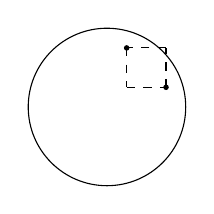
\begin{tikzpicture}
          \draw (0, 0) circle [radius=1];
          \fill (0.25,0.75) circle (1pt);
          \fill (0.75,0.25) circle (1pt);
          \draw[dashed] (0.25,0.75) -- (0.25, 0.25);
          \draw[dashed] (0.25,0.25) -- (0.75, 0.25);
          \draw[dashed] (0.75,0.25) -- (0.75, 0.75);
          \draw[dashed] (0.75,0.75) -- (0.25, 0.75);
    \end{tikzpicture}\]
    }
    \definition[Ориентированная граница прямоугольника $P$]{
    Петля $\gamma$, обходящая границу $P = [a, b] \times [c, d]$ против часовой стрелки, то есть вот так:
    \[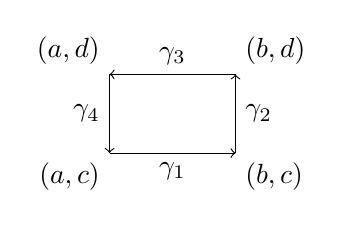
\begin{tikzpicture}
          \draw (0,0) node[below left] {$(a, c)$};
          \draw (0,1) node[above left] {$(a, d)$};
          \draw (1.6,0) node[below right] {$(b, c)$};
          \draw (1.6,1) node[above right] {$(b, d)$};

          \node at (0.8,0) [below] {$\gamma_1$};
          \node at (1.6,0.5) [right] {$\gamma_2$};
          \node at (0.8,1) [above] {$\gamma_3$};
          \node at (0,0.5) [left] {$\gamma_4$};

          \draw[->] (0,0) -- (1.6, 0);
          \draw[->] (1.6,0) -- (1.6, 1);
          \draw[->] (1.6,1) -- (0, 1);
          \draw[->] (0,1) -- (0, 0);
    \end{tikzpicture}\]
    $\gamma = \gamma_1 \oplus \gamma_2 \oplus \gamma_3 \oplus \gamma_4$.
    }
    Для прямоугольника $P$ будем обозначать за $\partial P$ в зависимости от контекста либо границу $P$, как топологического подмножества $\R^2$, либо путь, обходящий границу $P$ против часовой стрелки.
    \corollary[Дополнение к~(\cref{integral-along-path})]{
        Если $G$ --- удобная область на плоскости, то к трём эквивалентным условиям~(\cref{integral-along-path}) можно добавить
    \numbers{
    \item[4.] $\forall P \subset G: \int\limits_{\partial P}\Phi = 0$.
    }
    \provehere{
    $(3) \then (4)$ ясно, докажем $(4) \then (1)$.

    Пусть $x_0 \in G$ --- центр удобной области, определим $F(x) = \int\limits_{\delta}\Phi$, где $\delta$ --- это либо $\delta_1 \coloneqq \gamma_1 \oplus \gamma_2$ либо $\delta_2 \coloneqq \gamma_4^- \oplus \gamma_3^-$ (вне зависимости от выбора $\delta$ получится одно и то же).
        \[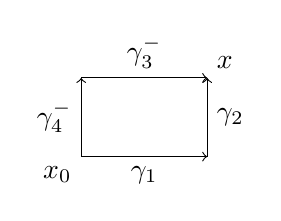
\begin{tikzpicture}
              \draw (0,0) node[below left] {$x_0$};
              \draw (1.6,1) node[above right] {$x$};

              \node at (0.8,0) [below] {$\gamma_1$};
              \node at (1.6,0.5) [right] {$\gamma_2$};
              \node at (0.8,1) [above] {$\gamma_3^-$};
              \node at (0,0.5) [left] {$\gamma_4^-$};

              \draw[->] (0,0) -- (1.6, 0);
              \draw[->] (1.6,0) -- (1.6, 1);
              \draw[<-] (1.6,1) -- (0, 1);
              \draw[<-] (0,1) -- (0, 0);
        \end{tikzpicture}\]
    Далее, чтобы проверить $\der{}{x_1}F = f_1$ и $\der{}{x_2}F = f_2$, воспользуемся подходящим представлением: пусть орт выглядит так: % "орт" --- это один, что тут имеется ввиду? "пусть орты расположены так"?
        \[\begin{tikzpicture}[scale=1]
            \draw[->](0,0) -- (0,1) node [below left] {$x_1$};
            \draw[->](0,0) -- (1,0) node [below left] {$x_2$};
        \end{tikzpicture}\]
        тогда для проверки $\der{}{x_1}F = f_1$ удобно воспользоваться определением $F$ через $\delta_1$, для проверки $\der{}{x_2}F = f_2$ --- определением через $\delta_2$. Далее повторяем рассуждение из (\cref{integral-along-path}).
    }
    }
    Пусть $\Phi = \sum\limits_{j = 1}^{n}f_j(x)\d x_j$ --- непрерывная дифференциальная форма в области $G \subset \R^n$.
    \definition[Форма $\Phi$ точна]{Существует первообразная $F$ в $G: \d F = \Phi$. }
    \definition[Форма $\Phi$ замкнута]{ Форма $\Phi$ локально точна ($\forall x_0 \in G: \exists U \ni x_0$: $\Phi\big|_U$ точна). }
    Понятно, что точная форма замкнута, но точность из замкнутости не следует: чуть позднее мы определим $\d z$, и покажем, что $\frac{\d z}{z}$ --- замкнутая, но не точная форма на $\C \sm \{0\}$
    \theorem{
    Пусть $\Phi$ --- дифференциальная форма в области $G \subset \R^n$.
        Следующие условия эквивалентны:
    \numbers{
    \item $\Phi$ замкнута.
    \item $\forall x_0 \in G: \exists V \ni x_0: \forall$ кусочно-гладкого замкнутого пути $\gamma$ с носителем в $V$: $\int\limits_{\gamma}\Phi = 0$.
    }
    Если $n = 2$, то дополнительно появляются ещё два условия:
    \numbers{
    \item[3.] $\forall z \in G: \exists \underset{\ni z}{V_z} \subset G: \forall P \subset V_z: \int\limits_{\partial P}\Phi = 0$.
    \item[4.] $\forall P \subset G: \int\limits_{\partial P}\Phi = 0$.
    }
    \provehere{
    Докажем, что $(3) \then (4)$, остальное уже доказано выше.

    Заметим, что границу прямоугольника $P$ можно представить, как сумму границ четырёх прямоугольников вдвое меньшего диаметра:
        \[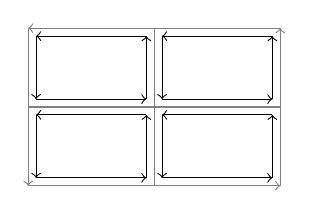
\begin{tikzpicture}
              \draw[->,color=gray] (0,0) -- (3.2, 0);
              \draw[->,color=gray] (3.2,0) -- (3.2, 2);
              \draw[->,color=gray] (3.2,2) -- (0, 2);
              \draw[->,color=gray] (0,2) -- (0, 0);
              \draw[color=gray] (0,1) -- (3.2,1);
              \draw[color=gray] (1.6,0) -- (1.6,2);
              \foreach \x/\y in {0/0,1.6/0,0/1,1.6/1} {
                  \draw[->] ({\x+0.1},{\y+0.1}) -- ({\x+1.5}, {\y+0.1});
                  \draw[->] ({\x+1.5},{\y+0.1}) -- ({\x+1.5}, {\y+0.9});
                  \draw[->] ({\x+1.5},{\y+0.9}) -- ({\x+0.1}, {\y+0.9});
                  \draw[->] ({\x+0.1},{\y+0.9}) -- ({\x+0.1}, {\y+0.1});
              }
        \end{tikzpicture}\]

    Таким образом, чтобы доказать, что интеграл по границе большого прямоугольника $P$ нулевой, разобьём его на достаточно маленькие прямоугольники, по ним-то интеграл нуль.
    Чтобы это формализовать, вспомним лемму Лебега о покрытии:
    \theorem[Лемма Лебега]{
    Пусть $K$ --- компакт в метрическом пространстве, $\{U_j\}_{j \in J}$ --- открытое покрытие компакта $K$. Тогда $\exists \delta > 0: \forall A \subset K: \diam A < \delta \then \exists j \in J: A \subset U_j$.
    }
    Применяя лемму Лебега для покрытия $P$ окрестностями $\{V_z\}_{z \in P}$, получим такое число $\delta$. Теперь надо разбить границу прямоугольника $P$ в сумму границ прямоугольников диаметра меньше $\delta$, а посылка теоремы говорит, что интеграл по ним уже нуль.
    }
    }
    \section{Операторы $\der{}{z}$ и $\der{}{\overline{z}}$}
    Как известно, $\C = \defset{x + iy}{x, y \in \R}$, то есть $\forall z \in \C: z = x + iy$, аналогично $\overline{z} = x - iy$.

    Рассмотрим $z$ и $\overline{z}$, как функции $\R^2 \map \C, (x, y) \mapsto x \pm iy$.
    Теперь $\d z = \d x + i \d y$ и $\d \overline{z} = \d x - i \d y$ образуют базис в пространстве дифференциальных форм (тех, которые не зависят от точки), обратное преобразование выглядит так:
    \[\all{\d x = \frac{\d z + \d \overline{z}}{2} \\ \d y = \frac{\d z - \d \overline{z}}{2i}}\]
    Рассмотрим форму $\Phi: \R^2 \map \C, \Phi(x, y) = \alpha(x, y)\d x + \beta(x, y)\d y$.
    Перепишем её в новом базисе:
    \[\Phi(x, y) = \frac{\alpha(x, y)}{2}(\d z + \d \overline{z}) + \frac{\beta(x, y)}{2i}(\d z - \d\overline{z}) = \frac{\alpha(x, y) - i \beta(x, y)}{2}\d z + \frac{\alpha(x, y) + i \beta(x, y)}{2}\d \overline{z}\]
    Теперь пусть $\Phi$ --- точная форма, то есть $\Phi = \d F$, и тогда $\alpha(x, y) = \der{}{x}F(x, y)$ и $\beta(x, y) = \der{}{y}F(x, y)$. Теперь
    \[\d F = \frac{1}{2}\left(\der{F}{x} - i\der{F}{y}\right)\d z + \frac{1}{2}\left(\der{F}{x} + i \der{F}{y}\right)\d \overline{z}\]
    \definition[$\der{F}{z}$]{
    Коэффициент, стоящий перед $\d z$, то есть $\frac{1}{2}\left(\der{F}{x} - i\der{F}{y}\right)$.
    }
    \definition[$\der{F}{\overline{z}}$]{
    Коэффициент, стоящий перед $\d \overline{z}$, то есть $\frac{1}{2}\left(\der{F}{x} + i \der{F}{y}\right)$.
    }
    Иначе говоря, мы ввели операторы $\der{}{z} \bydef \frac{1}{2}\left(\der{}{x} - i\der{}{y}\right)$ и $\der{}{\overline{z}} \bydef \frac{1}{2}\left(\der{}{x} + i \der{}{y}\right)$ так, что \[\d F = \der{}{z}F\d z + \der{}{\overline{z}}F\d\overline{z}\]
    \subsection{Связь с голоморфными функциями}
    Пусть $F = u + iv$, где $u, v: \R^2 \map \R$.
    Запишем
    \[\der{F}{\overline{z}} = \frac{1}{2}\left(\der{u}{x} + i\der{v}{x} + i\left(\der{u}{y} + i\der{v}{y}\right)\right) = \frac12\left(\left(\der{u}{x} - \der{v}{y}\right) + i\left(\der{v}{x} + \der{u}{y}\right)\right)\]
    В правой части равенства получились выражения из уравнений Коши --- Римана.
    \fact{
    Вещественные функции $u, v$ удовлетворяют уравнениям Коши --- Римана $\iff \der{(u + iv)}{\overline{z}} \equiv 0$.
    }
    \fact{
    $F$ голоморфна $\iff \d F = \der{F}{z}\d z$.
     При этом $\der{F}{z}$ есть производная $F$ по комплексному аргументу.
        \provehere{
            Функция дифференцируема по комплексному аргументу $\iff$ её дифференциал --- умножение на комплексное число.
        }
    }
    В основном нас будут интересовать дифференциальные формы вида $\phi(z)\d z$, где $\phi$ --- произвольная функция.

    Выясним, когда у формы $\phi(z)\d z = \phi(z)\d x + i\phi(z)\d y$ имеется первообразная, то есть функция $g: \der{g}{x} = \phi, \der{g}{y} = i\phi$.
    Заметим, что $\der{g}{z} = \frac{1}{2}(\phi - i(i\phi)) = \phi$ и $\der{g}{\overline{z}} = \frac{1}{2}(\phi + i(i\phi)) = 0$.
    \statement{
    Форма $\phi\d z$ имеет первообразную $g \iff g$ голоморфна, и $g' = \phi$.
    }
    \theorem[Коши]{\label{cauchey-theorem}
    Если $g: G \map \C$ --- голоморфная функция (область $G \subset \C$), то форма $g(z)\d z$ замкнута.
    \provehere{Потом.}
    }
    \counterexample[Глобально первообразной может не быть]{
        Пусть $G = \C \sm \{0\}, g: G \map \C, g: z \mapsto \frac{1}{z}$.

    По теореме Коши у $g$ имеется локальная первообразная --- комплексный логарифм --- но глобально определить не получится.
        Пусть $\Gamma = \partial \mathbb{T}$ --- комплексная окружность, ориентируем её против часовой стрелки, а именно, рассмотрим стандартный обход окружности $\alpha: [0, 2\pi] \map \C,\: \alpha: \phi \mapsto e^{i\phi}$.
    Теперь убедимся, что форма не точна:
    \[\int\limits_{\alpha}\phi = \int\limits_{\alpha}\frac{\d z}{z} = \int\limits_{0}^{2\pi}\frac{\left(e^{it}\right)'}{e^{it}}\d t =\int\limits_{0}^{2\pi}\d t = 2\pi i \ne 0\]
    }
    Для будущих применений также определим ориентированную против часовой стрелки границу $B_r(z_0)$, это путь $\beta(t) = z_0 + r e^{i t}$ для $t \in [0, 2\pi]$.

    \example{
    Пусть $z_0, w \in \C, r \in \R_{> 0}$, $|w - z_0| \ne r$, пусть путь $\gamma$ обходит границу $B_r(z_0)$ против часовой стрелки:
        \[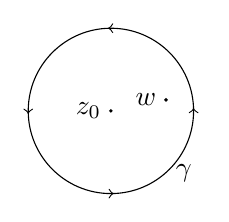
\begin{tikzpicture}[scale=0.7]
              \draw (0, 0) circle [radius=1.5];
              \fill (0, 0) circle (1pt) node[left] {$z_0$};
              \fill (1, 0.2) circle(1pt) node[left] {$w$};
              \draw[->] (1.5,-0.05) -- (1.5,0.05);
              \draw[->] (-1.5,0.05) -- (-1.5,-0.05);
              \draw[->] (0.05,1.5) -- (-0.05,1.5);
              \draw[->] (-0.05,-1.5) -- (0.05,-1.5);
              \node[below right] at (1,-0.8) {$\gamma$};
            \end{tikzpicture}\]
        Тогда, оказывается, (посчитаем чуть позже):
    \[\int\limits_{\gamma}\frac{\d z}{z - w} = \all{0,&|z - w| > r \\ 2\pi i,&|z - w| < r}\tag{$\circ$}\label{circle-integral}\]
    Грубой силой этот интеграл посчитать непросто, так как $w$ находится где угодно --- внутри или снаружи круга --- а интеграл, оказывается, зависит только от этих двух альтернатив.
    }
    \theorem[Основная оценка интеграла вдоль пути]{
        Пускай $\Phi = \sum\limits_{j=1}^n f_j\d x_j$ --- непрерывная дифференциальная форма в области $G \subset \R^n$, а $\gamma: [a, b] \map G$ --- кусочно-гладкий путь, $K \coloneqq \Image(\gamma) \subset G$.

    Тогда $\abs{\int\limits_{\gamma}\Phi} \le \underbrace{\sup\limits_{x \in K}\left(\sum\limits_{j = 1}^{n}|f_j(x)|^2\right)^{\nicefrac{1}{2}}}_{\eqqcolon A}\cdot l(\gamma)$.
    \provehere{
    Считаем, что $\gamma$ --- гладкий путь, иначе нужно разбить на кусочки гладкости.
    \[\abs{\int\limits_{\gamma}\Phi} = \abs{\int\limits_{a}^{b}\sum\limits_{j = 1}^{n}f_j\left(\gamma(t)\right)\gamma_j'(t)\d t} \underset{\text{КБШ}}\le \int\limits_{a}^{b}\left(\sum\limits_{j = 1}^{n}|f_j(\gamma(t))|^2\right)^{\nicefrac{1}{2}} \cdot \left(\sum\limits_{j = 1}^{n}|\gamma_j'(t)|^2\right)^{\nicefrac{1}{2}}\d t \le A \cdot \underbrace{\int\limits_{a}^{b}\left(\sum\limits_{j = 1}^{n}|\gamma_j'(t)|^2\right)^{\nicefrac{1}{2}}\d t}_{l(\gamma)}\]
    }
    }
    \newlection{1 марта 2024 г.}
    Рассмотрим дифференциальную форму $\Phi = F(z)\d z$, где $F$ --- непрерывная функция в $G \subset \C$.
    Пусть $\gamma: [a, b] \map G$ --- плоский путь.

    Расписав $\Phi(z) = F(z)\d x + i F(z)\d y$ и применив основную оценку интеграла вдоль пути, получаем
    \[\abs{\int\limits_{\gamma}\Phi} \le \max\limits_{z \in K}\sqrt{|F(z)|^2 + |F(z)|^2} \cdot l(\gamma) = \sqrt{2}\max\limits_{z \in K}|F(z)| \cdot l(\gamma)\]
    Эта оценка вызывает некоторую неудовлетворённость: кажется, что $\sqrt{2}$ здесь лишний.
    И это действительно правда: можно расписать интеграл аккуратнее.

    Пусть $\gamma = \gamma_1 + i\gamma_2$, тогда по определению
    \[\int\limits_{\gamma}\Phi = \int\limits_{a}^{b}F(\gamma(t))\cdot \gamma_1'(t) + i F(\gamma(t))\cdot \gamma_2'(t)\d t = \int\limits_{a}^{b}F(\gamma(t)) \cdot \gamma'(t)\d t\]
    Таким образом, интеграл от комплексной формы вдоль пути имеет более простое представление, и оно легко поддаётся более плотной оценке:
    \[\abs{\int\limits_{\gamma}\Phi} \le \int\limits_{a}^{b}|F(\gamma(t))| \cdot |\gamma'(t)|\d t \le \max\limits_{z \in K}|F(z)| \underbrace{\int\limits_{a}^{b}|\gamma'(t)|\d t}_{l(\gamma)}\]

    Посчитаем анонсированный на предыдущей лекции интеграл~\eqref{circle-integral}.
    Пусть $z_0, w \in \C$, $r > 0$.
    \bullets{
        \item Сначала рассмотрим случай $|w - z_0| < r$.
        Заметим, что, согласно основной оценке интеграла, если коэффициенты равномерно стремятся к какому-то значению и интегралы ограничены, то предельный интеграл тоже сходится.

        Запись ниже $\int\limits_{|z - z_0| = r}$, и вообще все аналогичные записи, которые встретятся в дальнейшем, по умолчанию означают, что граница соответствующего множества (в данном случае --- круга) обходится стандартным образом, то есть против часовой стрелки.
        \multline{\int\limits_{|z - z_0| = r}\frac{\d z}{z - z_0 - (w - z_0)} = \int\limits_{|z - z_0| = r}\frac{1}{z - z_0}\frac{1}{1 - \frac{w - z_0}{z - z_0}}\d z =\\= \int\limits_{|z - z_0| = r}\frac{1}{z - z_0}\left(1 + \frac{w - z_0}{z - z_0} + \left(\frac{w - z_0}{z - z_0}\right)^2 + \dots\right)\d z \circlesign{=}}
        На слагаемые из ряда имеется равномерная по $z$ оценка: $\abs{\frac{w - z_0}{z - z_0}} \le \frac{|w - z_0|}{r} < 1$, и по теореме Вейерштрасса функциональный ряд сходится.
        Значит, сумму можно вынести из-под интеграла
        \[\circlesign{=}\int\limits_{|z - z_0| = r}\frac{1}{z - z_0}\d z + \sum\limits_{j = 1}^{\infty}\ \int\limits_{|z - z_0| = r}\frac{(w - z_0)^j}{(z - z_0)^{j+1}}\d z \circlesign{=}\]
        Первое слагаемое мы умеем брать, а у каждого слагаемого из остальной суммы имеется первообразная: $\frac{1}{(z - z_0)^{j+1}} = -\frac{1}{j}\left(\frac{1}{(z - z_0)^{j}}\right)'$
        \[\circlesign{=}\int\limits_{|z - z_0| = r}\frac{1}{z - z_0}\d z = \int\limits_{0}^{2\pi}\frac{r i e^{it}}{r e^{it}}\d t = 2 \pi i\]
    \item Теперь разберёмся со случаем $|w - z_0| > r$.
        \[\int\limits_{|z - z_0| = r}\frac{\d z}{z - z_0 - (w - z_0)} = -\frac{1}{w - z_0}\int\limits_{|z - z_0| = r}\frac{\d z}{1 - \frac{z - z_0}{w - z_0}} = -\frac{1}{w - z_0}\sum\limits_{j = 0}^{\infty}\ \int\limits_{|z - z_0| = r}\frac{(z - z_0)^j}{(w - z_0)^j}\d z\]
    Аналогично предыдущему случаю, ряд сходится абсолютно, поэтому сумму опять можно вынести из под интеграла, и в данном случае всё ещё проще: каждое слагаемое имеет первообразную, там нет отрицательных степеней $z$, поэтому вся сумма обращается в нуль.
    }
    Пусть $\Phi = f_1 \d x_1 + \dots + f_n \d x_n$ --- непрерывная дифференциальная форма в некоторой области $G \subset \R^n$.
    \theorem{
    	\label{cross-partial}
    Если все функции $f_j \in C^1$, то следующие условия эквивалентны:
    \bullets{
    \item $\Phi$ замкнута.
    \item $\forall 1 \le i, j \le n: \der{f_i}{x_j} = \der{f_j}{x_i}$ --- <<накрест взятые частные производные равны>>.
    }
    \provenumbers{
    \item[$\then$] Выберем $x \in G$, так как форма замкнута, то $\exists U \ni x: \Phi$ имеет первообразную $F: U \map \R$.
    Тем самым, $f_i = \der{F}{x_i}$, и так как $f_i \in C^1$, то действительно $\der{f_j}{x_i} = \frac{\partial^2F}{\partial x_i \partial x_j} = \frac{\partial^2F}{\partial x_j \partial x_i} = \der{f_i}{x_j}$.
    \item[$\when$] Сначала приведём доказательство случая $n = 2$.
        В таком случае $\Phi = f\d x + g \d y$.

        Согласно посылке, $h \coloneqq \der{f}{y} = \der{g}{x}$.
        Кстати, равенство слева равносильно одному из эквивалентных уравнений Коши --- Римана.

        Рассмотрим произвольный $P = [a, b] \times [c, d] \subset G$, и докажем, что $\int\limits_{\partial P}\Phi = 0$.
        \[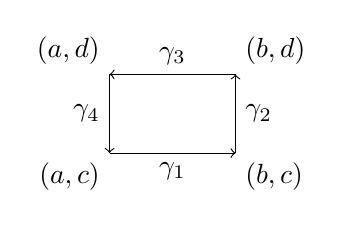
\begin{tikzpicture}
              \draw (0,0) node[below left] {$(a, c)$};
              \draw (0,1) node[above left] {$(a, d)$};
              \draw (1.6,0) node[below right] {$(b, c)$};
              \draw (1.6,1) node[above right] {$(b, d)$};

              \node at (0.8,0) [below] {$\gamma_1$};
              \node at (1.6,0.5) [right] {$\gamma_2$};
              \node at (0.8,1) [above] {$\gamma_3$};
              \node at (0,0.5) [left] {$\gamma_4$};

              \draw[->] (0,0) -- (1.6, 0);
              \draw[->] (1.6,0) -- (1.6, 1);
              \draw[->] (1.6,1) -- (0, 1);
              \draw[->] (0,1) -- (0, 0);
        \end{tikzpicture}\]
        То, что мы увидим сейчас, является первым заходом на \emph{формулу Остроградского --- Гаусса}.
        Функция $h$ непрерывна, и можно записать на неё интеграл Лебега:  $\int\limits_{P}h(x, y)\d x \d y$. % "записать на неё"?
        Теперь, применяя теорему Фубини, раскладываем интеграл в сумму повторных:
        \multline{\int\limits_{\gamma_3^-}f(\_, d)\d x + \int\limits_{\gamma_1^-}f(\_, c)\d x = \int\limits_{a}^{b}\left[f(x, d) - f(x, c)\right]\d x = \int\limits_{a}^{b}\left(\int\limits_{c}^{d}\der{f}{y}\d y\right)\d x
            =\\= \int\limits_{P}h(x, y)\d x \d y =\\=
            \int\limits_{c}^{d}\left(\int\limits_{a}^{b}\der{g}{x}\d x\right)\d y = \int\limits_{c}^{d}\left[g(b, y) - g(a, y)\right]\d y = \int\limits_{\gamma_2}g(b, \_)\d y + \int\limits_{\gamma_4}g(a, \_)\d y}
        Итого, $\int\limits_{\gamma_3^-}f(\_, d)\d x + \int\limits_{\gamma_1^-}f(\_, c)\d x = \int\limits_{\gamma_2}g(b, \_)\d y + \int\limits_{\gamma_4}g(a, \_)\d y$, откуда действительно $\int\limits_{\gamma}\Phi = 0$.
    \item[$\when$] Теперь приведём альтернативное доказательство индукцией по $n$.

    \underline{База:} Случай $n = 1$ тривиален: теорема Ньютона --- Лейбница говорит, что у непрерывной функции есть первообразная.

    \underline{Переход:} Пусть $n > 1$, и для $n - 1$ теорема доказана.
    Рассмотрим $a \in G$, и возьмём прямоугольный параллелепипед со сторонами, параллельными осям координат $P$ такой, что $a \in \Int P$.
        Докажем, что на $P$ у $\Phi$ есть первообразная.

    Построим $g(x_1, \dots, x_n) = \int\limits_{a_1}^{x_1}f_1(t, x_2, \dots, x_n)\d t$. Обозначим $\phi_j \coloneqq \der{g}{x_j}$.
        Заметим, что $\phi_1 = \der{g}{x_1} = f_1$.

    Теперь рассмотрим форму $\Psi(x_1, \dots, x_n) = \phi_1 \d x_1 + \dots + \phi_n \d x_n$.
        Эта форма имеет первообразную $g$ на параллелепипеде $P$.

    Теперь посмотрим на $\Phi - \Psi \eqqcolon h_1 \d x_1 + \dots + h_n \d x_n$.
        По построению $h_1 = 0$.
        По условию накрест взятые частные производные равны у $\Phi$, и они равны у $\Psi$, так как у неё есть первообразная.
    Значит, это же верно и для разности, в частности, $\der{h_i}{x_1} = \der{h_1}{x_i} = 0$.
        Иными словами, $\forall i: h_i$ не зависит от $x_1$.

    А раз так, то на $\Phi - \Psi$ можно смотреть, как на форму $(n-1)$-й переменной, и применить индукционное предположение.

    \note{
        Тут есть некоторый обман: производные $\der{\phi_i}{x_j}$ могут просто не существовать.

        Попробуем обойти его так: пусть $\beta \in C^\infty$, с компактным носителем.
        Выберем аппроксимативную единицу $\beta_t(x) = \frac{1}{t^n}\beta(\frac{x}{t})$.

        Назначим $f_k^{(t)} = f_k * \beta_t$, $f_k^{(t)} \underset{t \to 0}\rightrightarrows f_k$.

        Далее у формы $\Phi^{(t)}$ коэффициенты $h_k^{(t)}$ не зависят от $x_1$. А раз они равномерно стремятся к $h_k$, то и они не зависят от $x_1$.
        \comment{
        Это было произнесено устно, я наверняка что-то не так записал.
        }
        % Там было что-то про возьмём малый палраллелепипед и большой (и малое t) так, чтобы при вычислении свётки из малого параллелепипеда мы не выходили за большой, как-то так объясняли равномерную сходимость f_k^{(t)} на всём P. 
    }
    }
    }
    \theorem[Коши]{
    Пусть $F$ --- голоморфная функция в открытом множестве $G \subset \C$. Тогда дифференциальная форма $F(z)\d z$ замкнута, то есть локально $\exists S: S'(z) = F(z)$.
        \note{
        Теорема совсем проста, если заранее предположить, что $F'(z)$ непрерывна (а так в итоге и должно получиться, так как $F$ --- аналитична~(\cref{analytic-is-holomorphic})).
        В таком случае имеется следующее более простое доказательство.
        \provehere{
            Надо проверить второе уравнение Коши --- Римана: $\forall z \in \C: \der{F}{y}(z) = i \der{F}{x}(z)$ (первое выполнено, так как накрест-взятые частные производные равны).

            Поскольку $F(z)\d z = F(z)\d x + i F(z)\d y$, утверждение эквивалентно (согласно (\cref{cross-partial})) тому, что $\forall z \in \C: \der{F}{y}(z) = i \der{F}{x}(z)$.
        Пусть $F(z) = u(x, y) + i v(x, y)$.
        \[\der{u}{y} + i\der{v}{y} \underset{?}= i\left(\der{u}{x} + i\der{v}{x}\right)\]
        то есть $\der{u}{y} = -\der{v}{x}$ и $\der{v}{y} = \der{u}{x}$.
        \comment{Я вообще не понял, что произошло.}
        }
        }
        Теперь докажем теорему Коши вне предположения непрерывности производной.
    \provehere{
    Докажем от противного: пусть форма $F(z)\d z$ не замкнута, $\exists P_0 \subset G: \alpha = \int\limits_{\partial P_0}F(z)\d z \ne 0$.

    Будем потихонечку делить этот прямоугольник на четыре равные части: пусть $P_0 = Q_1 \cup Q_2 \cup Q_3 \cup Q_4$.
        \[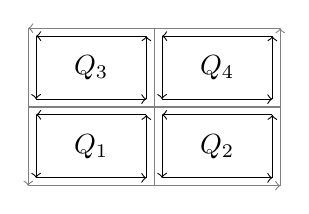
\begin{tikzpicture}
              \draw[->,color=gray] (0,0) -- (3.2, 0);
              \draw[->,color=gray] (3.2,0) -- (3.2, 2);
              \draw[->,color=gray] (3.2,2) -- (0, 2);
              \draw[->,color=gray] (0,2) -- (0, 0);
              \draw[color=gray] (0,1) -- (3.2,1);
              \draw[color=gray] (1.6,0) -- (1.6,2);
              \foreach \x/\y/\i in {0/0/1,1.6/0/2,0/1/3,1.6/1/4} {
                  \draw[->] ({\x+0.1},{\y+0.1}) -- ({\x+1.5}, {\y+0.1});
                  \draw[->] ({\x+1.5},{\y+0.1}) -- ({\x+1.5}, {\y+0.9});
                  \draw[->] ({\x+1.5},{\y+0.9}) -- ({\x+0.1}, {\y+0.9});
                  \draw[->] ({\x+0.1},{\y+0.9}) -- ({\x+0.1}, {\y+0.1});
                  \node at ({\x + 0.8}, {\y + 0.5}) {$Q_{\i}$};
              }
        \end{tikzpicture}\]
    Модуль интеграла по границе по крайней мере одного из $Q_i$ хотя бы $\frac{|\alpha|}{4}$.
        Назовём этот прямоугольник $P_1$, и продолжим процесс.
        Получим систему вложенных замкнутых прямоугольников $P_0 \supset P_1 \supset \dots$, таких, что $\abs{\int\limits_{\partial P_k}F(z)\d z} \ge \frac{|\alpha|}{4^k}$.
        При этом $l(\partial P_k) = 2^{-k}l(\partial P_0)$, и $\diam (P_k) = 2^{-k} \diam(P_0)$.

    Имеется ровно одна точка $z_0$ в пересечении $\bigcap\limits_{k \ge 0}P_k$.
        Воспользуемся условием того, что $F$ голоморфна в точке $z_0$: $F(z) = F(z_0) + F'(z_0)(z - z_0) + \underbrace{\psi(z)}_{o(|z - z_0|)}$

    Зафиксируем $\eps > 0$. $\exists \delta > 0: |z - z_0| < \delta \then |\psi(z)| \le \eps|z - z_0|$.
        Пусть $k$ настолько велико, что $\diam P_k < \delta$.
    \[\int\limits_{\partial P_k}F(z)\d z = \int\limits_{\partial P_k}[F(z_0) + F'(z_0)(z -z_0)]\d z + \int\limits_{\partial P_k}\psi(z)\d z\]
    Первый интеграл обнуляется, так как это линейная функция по $z$, у неё есть первообразная.
        Оценивая второй интеграл, получаем \[\frac{|\alpha|}{4^k} \le \abs{\int\limits_{\partial P_k}\psi(z)\d z} \le \eps\diam P_k \cdot l(\partial P_0) = \eps\cdot2^{-k}\diam P_0 \cdot 2^{-k}l(\partial P_0) = 4^{-k}\eps \cdot \diam P_0 \cdot l(\partial P_0)\]
    Выбирая довольно маленький $\eps$, получаем, что $|\alpha|$ меньше любого положительного числа.
    }
    }
    \theorem[Об устранимой особенности замкнутой дифференциальной формы]{\label{disposable-feature}
        Пускай $\Phi = f \d x + g\d y$ --- непрерывная дифференциальная форма в области $G \subset \C$.

        Если $z_0 \in G$, и $\Phi$ замкнута в $G \sm \{z_0\}$, то $\Phi$ замкнута в $G$.
        \provehere{
            Докажем, что $\forall P \subset G: \int\limits_{\partial P}\Phi = 0$.
            Рассмотрим случаи.
        \bullets{
            \item Если $z_0 \notin P$, то интеграл нуль по условию.
            \item Если $z_0 \in \Int P$, то данный случай сводится к следующему: разобьём прямоугольник на два так, чтобы $z_0$ оказалось на границе:
            \[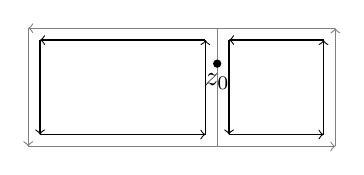
\begin{tikzpicture}[scale=1.5]
                  \draw[->,color=gray] (0,0) -- (2.6, 0);
                  \draw[->,color=gray] (2.6,0) -- (2.6, 1);
                  \draw[->,color=gray] (2.6,1) -- (0, 1);
                  \draw[->,color=gray] (0,1) -- (0, 0);
                  \draw[color=gray] (1.6,0) -- (1.6,1);
                  \fill (1.6,0.7) circle (1pt) node[below] {$z_0$};
                  \foreach \x/\w in {0/1.6, 1.6/1} {
                      \draw[->] ({\x+0.1},{0.1}) -- ({\x+\w-0.1}, {0.1});
                      \draw[->] ({\x+\w-0.1},{0.1}) -- ({\x+\w-0.1}, {0.9});
                      \draw[->] ({\x+\w-0.1},{0.9}) -- ({\x+0.1}, {0.9});
                      \draw[->] ({\x+0.1},{0.9}) -- ({\x+0.1}, {0.1});
                  }
            \end{tikzpicture}\]
            \item Если $z_0 \in \partial P$, то отступим на $\eps$, интеграл по границе $P_\eps$ будет нулём: $\int\limits_{\partial P_\eps}\Phi = 0$. % Без картинки непонятно, что за $P_\eps$

        Заметим, что $\int\limits_{\partial P_\eps}\Phi \underset{\eps \to 0}\Map \int\limits_{\partial P}\Phi$, так как коэффициенты дифференциальной формы равномерно непрерывны в некоторой окрестности $P$.
            Значит, $\int\limits_{\partial P}\Phi = 0$. % Тут чего-то надо расписать про то, что две стороны сокращаются, а другие две стороны просто короткие, длины \eps
        }
        }
    }
    \theorem[Малая интегральная формула Коши]{\label{integral-form}
    Пусть $f$ --- голоморфна в области $G$, $B = B(z_0, r)$ --- круг, $\overline{B} \subset G$. Тогда $\forall z \in B$:
    \[f(z) = \frac{1}{2\pi i}\int\limits_{\partial B}\frac{f(\zeta)}{\zeta - z}\d \zeta\]
    \provehere{
    Докажем для некоего фиксированного $z \in B$.

        Рассмотрим функцию $g(\zeta) = \frac{f(z) - f(\zeta)}{z - \zeta}$.
        $g$ голоморфна в области $G \sm \{z\}$. Тем самым, $g(\zeta)\d \zeta$ --- замкнутая форма в $G \sm \{z\}$, а по теореме об устранимой особенности $g(\zeta)\d \zeta$ замкнута в $G$ (доопределим по непрерывности $g(z) \coloneqq f'(z)$).

        Но так как круг --- удобная область, то у $g$ имеется первообразная в некотором круге $B(z_0, r(1 + \eps))$ (где $\eps > 0$ настолько мал, что $B(z_0, r(1 + \eps)) \subset G$),

        Тем самым, $\int\limits_{|\zeta - z_0| = r}\frac{f(z) - f(\zeta)}{z - \zeta}\d \zeta = 0$, откуда \[\int\limits_{|\zeta - z_0| = r}\frac{f(\zeta)}{\zeta - z}\d \zeta = \int\limits_{|\zeta - z_0| = r}\frac{f(z)}{\zeta - z}\d \zeta = f(z)\cdot\int\limits_{|\zeta - z_0| = r}\frac{1}{\zeta - z}\d \zeta = 2\pi i \cdot f(z)\]
    }
    }
    \corollary[Теорема Коши]{\label{holomorphic-then-analytic}
    Если функция голоморфна в области $G \subset \C$, то $\forall z_0 \in G$ функция $f$ (в некоторой окрестности) раскладывается в некоторый степенной ряд $f(z) = \sum\limits_{n = 0}^{\infty}c_n(z - z_0)^n$, причём радиус сходимости хотя бы $\dist(z_0, \partial G)$.
    \provehere{
        Пусть $r \in (0, \dist(z_0, \partial G))$.
        Рассмотрим $B = B_r(z_0)$. Так как $B \subset G$, то для точки $z \in B$ получаем
    \multline{f(z) = 
    	\frac{1}{2\pi i}\int\limits_{|\zeta - z_0| = r}\frac{f(\zeta)}{\zeta - z}\d \zeta =
    	\frac{1}{2\pi i}\int\limits_{|\zeta - z_0| = r}\frac{f(\zeta)}{(\zeta - z_0) - (z - z_0)}\d \zeta =
    	\\
    	= \frac{1}{2\pi i}\int\limits_{|\zeta - z_0| = r}\frac{1}{\zeta - z_0}\cdot \frac{1}{1 - \frac{z - z_0}{\zeta - z_0}}f(\zeta)\d\zeta =
    	\frac{1}{2\pi i}\sum\limits_{j = 0}^{\infty}(z - z_0)^{j}\int\limits_{|\zeta - z_0| = r}\frac{f(\zeta)}{(\zeta - z_0)^{j+1}}\d \zeta}
        Абсолютная равномерная сходимость в круге радиус $r$ при $r < \dist(z_0, \partial G)$ имеется по тем же причинам, что и при доказательстве~\eqref{circle-integral}.

        Таким образом, мы получили степенной ряд, и так как коэффициенты степенного ряда, раз определены, не зависят от радиуса круга ($c_j = \frac{f^{(j)}(z_0)}{j!}$), то радиус сходимости данного ряда хотя бы $\dist(z_0, \partial G)$.
    }
    }
    \newlection{12 марта 2024 г.}
    \note{
        Интегральную форму Коши можно спокойно дифференцировать: так,
    \[\frac{\d}{\d z}f(z) = \frac{\d}{\d z}\left(\frac{1}{2\pi i}\int\limits_{|\zeta - z_0| = r}\frac{f(\zeta)}{\zeta - z}\d\zeta\right) = \frac{1}{2\pi i}\int\limits_{|\zeta - z_0| = r}\frac{f(\zeta)}{(\zeta - z_0)^2}\d\zeta\]
    В общем случае
        \[\frac{\d^k}{\d z^k}f(z) = \frac{\d^k}{\d z^k}\left(\frac{1}{2\pi i}\int\limits_{|\zeta - z_0| = r}\frac{f(\zeta)}{\zeta - z}\d\zeta\right) = \frac{k!}{2\pi i}\int\limits_{|\zeta - z_0| = r}\frac{f(\zeta)}{(\zeta - z_0)^{k+1}}\d\zeta\]
    }
    \definition[Целая (entire) функция]{
        Голоморфная функция, заданная в $\C$.
    }
    Выберем $z_0 = 0$.
    Согласно~(\cref{holomorphic-then-analytic}), получаем $f(z) = \sum\limits_{j = 0}^{\infty}c_j$, где $c_j = \frac{1}{2\pi i}\int\limits_{|\zeta| = r}\frac{f(\zeta)}{\zeta^{j+1}}\d\zeta$, причём имеется абсолютная сходимость везде в $\C$.
    \theorem{
    Если $f$ целая, и $|f(z)| = \bigO(z^N)$ при $|z| \underset{z \to \infty}\Map \infty$, то $f$ --- многочлен степени не более $N$.
    \provehere{
        Из определения $\bigO: \exists C, a \in \R: |f(z)| \le C|z|^n$ при $|z| > a$.

        Выберем $r > a$, и оценим: $|c_j| = \abs{\frac{1}{2\pi i}\int\limits_{0}^{2\pi}\frac{f\left(r e^{i\theta}\right)}{re^{i\theta}}i e^{i\theta}\d\theta} \le \frac{1}{2\pi}\int\limits_{0}^{2\pi}\frac{C r^N}{r^j}\d\theta = \frac{C r^N}{r^j}$.
        Получается, при $j > N: |c_j|$ меньше любого наперёд заданного положительного числа.
    }
    }
    \corollary[Теорема Лиувилля]{
        Ограниченная целая функция постоянна.
    }
    \corollary[Основная теорема алгебры]{
        $\forall p \in \C[z]: \deg p > 0 \then \exists z_0 \in \C: p(z_0) = 0$.
    \provehere{
        Пусть $p(z) = \sum\limits_{j = 0}^{N}c_j z^j$, где $N > 0$ и $c_N \ne 0$.

    Пойдём от противного: пусть $\forall z \in \C: p(z) \ne 0$.

    Рассмотрим $f(z) \coloneqq \frac{1}{p(z)}$.
        \bullets{
            \item С одной стороны, это целая функция: $\frac{\d}{\d z}f(z) = -\frac{p'(z)}{p(z)^2}$.

        \item С другой стороны, $f$ ограничена:
        оценим $|p(z)| \ge |z^N|\left(|c_N| - \sum\limits_{j = 0}^{N - 1}\frac{|c_j|}{|z|^{N-j}}\right)$, откуда для достаточно больших $|z|: |p(z)| \ge \frac{|c_N|}{2}|z|^N$.

        Тем самым, $p(z) \underset{|z| \to \infty}\Map \infty$, то есть $f(z) \underset{|z| \to \infty}\Map 0$.
            А при малых $|z|: f$ ограничена, как непрерывная функция на компакте.
        \item Тем самым, по теореме Лиувилля, $f \equiv \const$, то есть $p \equiv \const$. Противоречие, мы предполагали $\deg p > 0$.\qedhere
        }
    }
    }
    \theorem[Теорема о среднем]{
    Пусть $z_0 \in G, f: G \map \C$ голоморфна в $G$.
        Выберем $r < \dist(z_0, \partial G)$.
        Тогда \encircle{f(z_0) = \frac{1}{2\pi}\int\limits_{0}^{2\pi}f(z_0 + r e^{it})\d t}
        \provehere{
            Посчитаем $f(z_0)$ по интегральной формуле:
            \[f(z_0) = \frac{1}{2\pi i}\int\limits_{|\zeta - z_0| = r}\frac{f(\zeta)}{\zeta - z_0}\d\zeta = \frac{1}{2\pi i}\int\limits_{0}^{2\pi}\frac{f(z_0 + r e^{it})i r e^{it}}{r e^{it}}\d t = \frac{1}{2\pi}\int\limits_{0}^{2\pi}f(z_0 + r e^{it})\d t\]
        }
    }
    Это действительно среднее в обычном смысле: $f$ проинтегрирована по окружности по мере Лебега, и интеграл поделили на меру окружности.
    \theorem[Принцип максимума модуля]{
        Пусть $f: G \map \C$ --- непостоянная голоморфная функция. Тогда $|f|: z \mapsto |f(z)|$ не может достигать наибольшего значения при $z \in G$.
        \provehere{
            Пойдём от противного: пусть $\exists z_0 \in G: \forall z \in G: |f(z)| \le |f(z_0)|$.
            Выберем $r > 0: B(z_0, r) \subset G$, и докажем, что $|f|$ постоянна в $B(z_0, r)$.
            Пусть $\rho < r$, по теореме о среднем $|f(z_0)| = \frac{1}{2\pi}\abs{\int\limits_{0}^{2\pi}f(z_0 + \rho e^{it})\d t} \le \frac{1}{2\pi}\int\limits_{0}^{2\pi}\underbrace{|f(z_0 + \rho e^{it})|}_{\le |f(z_0)|}\d t$, причём равенство достигается только если $\forall t \in [0, 2\pi]: |f(z_0 + \rho e^{it})| = |f(z_0)|$ (если $\exists t_0 \in (0, 2\pi): |f(z_0 + \rho e^{it_0}| < |f(z_0)|)$, то по непрерывности $\exists \eps > 0: \forall t \in (t_0 - \eps, t_0 + \eps): |f(z_0 + \rho e^{it}| < |f(z_0)| - \eps$, то есть на промежутке $(t_0 - \eps, t_0 + \eps)$ интеграл строго меньше требуемого значения).
            \indentlemma{
                Пусть $f: G \map \C$ голоморфна, и $\exists z_0 \in G: f'(z_0) \ne 0$. Тогда $\exists U \ni z_0: f(z_0) \in \Int f(U)$.
            }{
                Теорема об обратной функции.
            }
            Тем самым, $\forall z \in B(z_0, r): f'(z) = 0$ (так как $|f(z)|$ --- максимум).

        Далее применяем теорему единственности, доказанную во II семестре: $f$ и константа, равная $|f(z_0)|$ совпадают на множестве с предельной точкой, значит, они совпадают везде в $G$.
        }
    }
    \corollary{
    Пусть $G$ --- ограниченная область, $f: \overline{G} \map \C$ голоморфна в $G$. Тогда $\forall z \in G: |f(z)| \le \max\limits_{\zeta \in \partial G}|f(\zeta)|$.
    \provehere{
    $f$ достигает своё наибольшее значение на компакте $\overline{G}$, но согласно принципу максимума, это значение достигается не внутри $G$.
    }
    }
    \section{Гармонические функции}
    Запишем теорему о среднем для $f: G \map \C$:
    \[f(z_0) = \int\limits_{1}{2\pi}(f(z_0) + r e^{it})\d t\]
    Пусть $f = u + iv$, где $u, v$ --- вещественные функции в $G$.
    Теорема о среднем говорит, что
    \[u(z_0) = \int\limits_{1}{2\pi}(u(z_0) + r e^{it})\d t \qquad v(z_0) = \int\limits_{1}{2\pi}(v(z_0) + r e^{it})\d t\]
    Так как $f$ аналитична, то в вещественном смысле $u, v \in C^{\infty}(G)$.

    Запишем уравнения Коши --- Римана:
    \[\der{u}{x} = \der{v}{y} \quad \der{u}{y} = -\der{v}{x}\]
    Дифференцируя второй раз, получаем \[\all{\frac{\partial^2 u}{\partial x^2} = \frac{\partial^2 v}{\partial x \partial y} \\ \frac{\partial^2 u}{\partial y^2} = -\frac{\partial^2 v}{\partial x \partial y}}\]
    Это так называемое \emph{уравнение Лапласа}: $\frac{\partial^2 u}{\partial x^2} + \frac{\partial^2 u}{\partial y^2} = 0$.

    Обобщим.
    Пусть $G \subset \R^n$ --- область, пусть $f \in C^2(G)$.
    \definition[$f$ --- гармоническая функция в $G$]{
        $\frac{\partial^2u}{\partial x_1^2} + \cdots + \frac{\partial^2u}{\partial x_n^2} = 0$.
    }
    Оператор $\Delta = \frac{\partial^2}{\partial x_1^2} + \cdots + \frac{\partial^2}{\partial x_n^2}$ называется \emph{оператором Лапласа}, и понятно, что гармонические функции --- в точности такие $u$, что $\Delta u = 0$.
    \statement{
    Если $u \in C^2(G)$, где область $G \subset \R^2$, то локально существует голоморфная $f: u = \Re f$.
        Иными словами, $\forall z_0 \in G: \exists U \ni z_0, \exists$ аналитическая $f: U \map \C: u = \Re f$.
    \provehere{
        Пусть $\phi \coloneqq \der{u}{x}, \psi \coloneqq -\der{u}{y}$. Тогда $\der{\phi}{x} - \der{\psi}{y} = 0$, то есть $\der{\phi}{x} = \der{\psi}{y}$ везде в $G$.

    Раз накрест-взятые частные производные совпадают, то дифференциальная форма $\phi \d x + \psi \d y$ замкнута, значит, локально имеется первообразная.
    \comment{Что-то я немного выпал, а что дальше?}
    }
    }
    \theorem[Морера]{
        Пусть $f: (G \subset \C) \map \C$ непрерывна.
        Следующие условия эквивалентны.
        \numbers{
        \item $f$ голоморфна в $G$.
        \item $f$ аналитична в $G$.
        \item Дифференциальная форма $f(z)\d z$ замкнута.
        }
    \provehere{
        $(1) \iff (2)$ уже доказано:~(\cref{analytic-is-holomorphic}) и~(\cref{holomorphic-then-analytic}).

    $(1) \then (3)$ доказано тоже:~(\cref{cauchey-theorem}).

    Докажем $(3) \then (2)$.
        Пусть $F$ --- первообразная формы $f(z)\d z$ в круге $B(z_0, r) \subset G$.
        $F$ голоморфна в $B(z_0, r)$, и $\forall z \in D: F'(z) = f(z)$.

    Значит, $F$ раскладывается в степенной ряд $F(z) = \sum\limits_{j = 0}^{\infty}a_j (z - z_0)^j$. Отсюда ${f(z) = \sum\limits_{j = 1}^{\infty}j a_j (z - z_0)^{j - 1}}$.
    }}
    \section{Первообразная от замкнутой формы вдоль непрерывного пути}
    \subsection{Наводящие предположения}
    Пусть $f\d x + g\d y$ --- непрерывная дифференциальная форма в $G$, предположим, что она точная: имеется первообразная $F$.

    Пусть $\gamma: [a, b] \map G$ --- кусочно-гладкий путь.
    Ранее было получено, что $\int\limits_{\gamma}f \d x + g \d y = F(\gamma(b)) - F(\gamma(a))$.

    Давайте обобщим интеграл вдоль пути: пусть $\gamma: [a, b] \map G$ --- произвольный непрерывный путь.
    Положим по определению $\int\limits_{\gamma}f \d x + g \d y \bydef F(\gamma(b)) - F(\gamma(a))$.

    Теперь пусть $f\d x + g\d y$ всего лишь замкнута.
    Выберем $a = t_0 < t_1 < \cdots < t_k = b$ так, что $\forall j: \gamma([t_j, t_{j+1}])$ лежит в области $G_j$, в которой у формы $f\d x + g\d y$ есть первообразная $F_j$.
    Попробуем определить
    \[\int\limits_{\gamma\big|_{[t_j, t_{j+1}]}}f \d x + g \d y \bydef F_j(\gamma(t_{j + 1})) - F_j(\gamma(t_j))\]
    и
    \[\int\limits_{\gamma}f \d x + g \d y \bydef \sum\limits_{j = 0}^{k - 1}F_j(\gamma(t_{j + 1})) - F_j(\gamma(t_j))\]
    Проблема в том, чтобы доказать, что определение корректно --- не зависит от выбора разбиения $a = t_0 < \dots < t_k = b$.
    \subsection{Требуемые свойства}
    Пусть $\Phi = f \d x + g \d y$ --- замкнутая форма в области $G \subset \C$, и $\gamma: [a, b] \map G$ --- путь.

    \definition[Первообразная формы $\Phi$ вдоль пути $\gamma$]{
    Такая функция $v: [a, b] \map G$:
    \bullets{
    \item $\forall t \in [a, b]: \exists U \ni \gamma(t), \eps > 0$ и найдётся первообразная $F$ для $\Phi$ на $U$, такая, что \[\forall \tau \in (t - \eps, t + \eps): v(\tau) = F(\gamma(\tau))\]
    }
    }
    \fact{
    Функция $v$, если существует, непрерывна на $[a, b]$.
    \provehere{
        Непрерывность в какой-то конкретной точке следует из непрерывности композиции $F \circ \gamma$.
    }
    }
    \theorem{\label{antiderivative-along-path}
    Первообразная замкнутой дифференциальной формы вдоль пути $\gamma$ всегда существует, и любые две отличаются на константу.
    \provehere{
    Сначала докажем существование. Для всех $t \in [a, b]$ выберем окрестность $U_t \coloneqq B(\gamma(t), r_t)$, где $r_t$ настолько мал, что в $U_t$ есть первообразная.

    Семейство $\{U_t\}_{t \in [a, b]}$ образуют открытое покрытие $\gamma([a, b])$.
        По лемме Лебега $\exists \eps > 0: \forall t \in [a, b]: B(\gamma(t), \eps)$ содержится в каком-то $U_{t'}$.
        Применяя теорему Кантора о ранвомерной непрерывности, получаем существование разбиения $a = t_0 < \dots < t_k = b$, такое, что $\gamma([t_j, t_{j + 1}])$ лежит в одном из $U_t$.

        Произвольно выберем $v(a)$.
        Построим $v\big|_{[t_j, t_{j+1}]}$ индукцией по $j$.

        \underline{База:} Пусть $\gamma([t_0, t_1]) \subset U_0$, и имеется первообразная $F_0$ на $U_0$. Определим $v(\tau) = F_0(\gamma(\tau))$ при $\tau \in [t_0, t_1]$.

        \underline{Переход:} Пусть $\gamma([t_j, t_{j+1}]) \subset U_j, F_j$ --- первообразная $\Phi$ на $U_j$.
        Найдётся такое $\delta > 0: \gamma([t_j - \delta, t_{j+1}]) \subset U_j$, значит, $U_j \cap U_{j-1} \ne \o$.
        Это пересечение связно, на нём имеются две первообразные, $F_{j-1}$ и $F_j$.

        Добавим константу к $F_j$ так, чтобы $F_j \equiv F_{j-1}$ при $t \in [t_j - \delta, t_j]$, и определим $v(\tau) = F_j(\gamma(\tau))$ при $\tau \in [t_j, t_{j+1}]$.
        Окрестность $U_j$ захватывает отрезок $[t_j - \delta, t_{j+1}]$, значит, для точек во внутренности выполнено условие из определения первообразной.

        Докажем единственность: рассмотрим точку $t \in [a, b]$. Найдутся два круга $U, V \ni \gamma(t)$, и первообразные $F, H$ формы $\Phi$ в этих окрестностях, такие, что $u(\tau) = F(\gamma(\tau))$ и $v(\tau) = H(\gamma(\tau))$ при $\tau$, достаточно близких к $t$.

    Тем самым, $u - v$ локально постоянна, но локально постоянная функция на связном множестве --- константа (прообраз любого элемента из образа открыто-замкнут).
    }
    }
    \newlection{15 марта 2024 г.}
    Теперь определим интеграл $\int\limits_{\gamma}\Phi = v(b) - v(a)$, где $v$ --- первообразная для $\Phi$ вдоль пути $\gamma$, получившаяся из~(\cref{antiderivative-along-path}).
    Теперь интеграл определён для любой замкнутой формы вдоль пути (однако для кусочно-гладкого пути интеграл~(\cref{piecewise-smooth-integral}) был определён для необязательно замкнутой формы).
    \properties[Свойства первообразной вдоль пути]{
    \item Аддитивность по дифференциальной форме: $\int\limits_{\gamma}(\Phi + \Psi) = \int\limits_{\gamma}\Phi + \int\limits_{\gamma}\Psi$.
    \item Аддитивность вдоль пути: $\int\limits_{\gamma_1 \oplus \gamma_2}\Phi = \int\limits_{\gamma_1}\Phi + \int\limits_{\gamma_2}\Phi$.
    \item Если $\gamma$ --- кусочно-гладкий путь, то определение совпадает со старым.
    \provehere{
    $\gamma'$ существует везде, кроме, может быть, конечного множества.

    При помощи леммы Лебега разобьём отрезок точками $a = t_0 < \dots < t_k = b$ так, что $\forall j < k: \exists U_j \supset \gamma([t_j, t_{j+1}])$ такая, что на $U_j$ найдётся первообразная $H_j$:
    \[\forall \tau \in [t_j, t_{j+1}]: F(\tau) = H_j(\gamma(\tau))\]
    И старый, и новый интегралы аддитивны вдоль пути. Несложно видеть, что в обеих определениях $\int\limits_{\gamma\big|_{[t_j, t_{j+1}]}}\Phi$ совпадают.
    }
    \item Так как путь $\gamma$ необязательно дифференцируем, то основную оценку интеграла вдоль пути распространить на новое определение проблематично: длины может не существовать.
    \item Пусть $\phi: [a, b] \map [c, d]$ --- гомеоморфизм, $\gamma: [a, b] \map G$ --- путь, тогда
    \[\int\limits_{\gamma}\Phi = \pm\int\limits_{\gamma \circ \phi}\Phi\]
    где знак зависит от того, возрастает $\phi$, или убывает.
    \provehere[Причина]{ Если $F$ --- первообразная $\Phi$ вдоль пути $\gamma$, то $F \circ \phi$ --- первообразная для $\Phi$ вдоль пути $\gamma \circ \phi$.
    }
    }
    \subsection{О гомотопности путей}
    Пусть $K = [0, 1] \times [a, b]$ --- квадрат гомотопии.
    \definition[Гомотопия]{Непрерывное отображение $\Gamma: K \map \C$.}
    Положим $\gamma_s \coloneqq \Gamma(s, \_)$.
    Как водится, $\gamma_0, \gamma_1$ --- два пути $[a, b] \map \C$, и существование $\Gamma$ по определению влечёт гомотопность этих путей.

    Пути $\gamma_0, \gamma_1: [a, b] \map G$ \emph{гомотопны в $G$}, если найдётся гомотопия $\Gamma: K \map G$.

    Будем говорить о гомотопности двух замкнутых путей $\gamma_1$ и $\gamma_2$ при условии существования гомотопии $\Gamma: K \map G$, соединяющей $\gamma_1$ и $\gamma_2$ в классе замкнутых путей: $\forall s \in [0, 1]: \Gamma(s, a) = \Gamma(s, b)$.

    Гомотопность путей --- отношение эквивалентности, также как и гомотопность замкнутых путей.

    \theorem{
        Пусть $F$ --- аналитическая функция в области $G$, а $\gamma_0$ и $\gamma_1$ --- замкнутые пути, гомотопные в $G$ (в классе замкнутых путей).
    Тогда $\int\limits_{\gamma_1}F \d z = \int\limits_{\gamma_2}F \d z$.
    \provehere{

    }
    }

    \definition[Односвязная область]{
        Область, в которой всякий замкнутый путь гомотопен постоянному.
        Иными словами, фундаментальная группа тривиальна.
    }
    \definition[Звёздная область $A \subset \R^n$]{
    Такая область, что для некоторого \emph{центра} $z_0 \in A$: $\forall z \in A: \defset{z_0 + s(z -z_0)}{s \in [0, 1]} \subset A$.
    }
    \[\begin{tikzpicture}
          \draw[dashed] (0.9, 0.5) -- (1, 2);
          \draw[dashed] (1, 2) -- (-0.2, 1);
          \draw[dashed] (-0.2, 1) -- (-2, 2);
          \draw[dashed] (-2, 2) -- (-1, 0.08);
          \draw[dashed] (-1, 0.08) -- (-2, -1);
          \draw[dashed] (-2, -1) -- (-0.4, -0.9);
          \draw[dashed] (-0.4, -0.9) -- (0.6, -2);
          \draw[dashed] (0.6, -2) -- (0.8, -0.7);
          \draw[dashed] (0.8, -0.7) -- (2, -0.2);
          \draw[dashed] (2, -0.2) -- (0.9, 0.5);
          \fill (0, 0) circle (1pt) node[right] {$z_0$};
          \fill (-1, 1) circle (1pt) node[right] {$z$};
          \draw[->] (0, 0) -- (-1, 1);
    \end{tikzpicture}\]
    \fact{Всякая звёздная область $A$ односвязна.
    \provehere{
    Прогомотопируем путь $\gamma: [a, b] \map A$ при помощи \begin{align*}\Gamma: [0, 1] \times [a, b] &\map K\\\tau, t &\mapsto z_0 \tau + (1 - \tau)\gamma(t)\qedhere\end{align*}
    }
    }
    \example[Неодносвязная область]{
    Пусть $A$ --- звёздная область, выкинем точку $w_0 \in A$.
        \[\begin{tikzpicture}
              \draw[dashed] (0.9, 0.5) -- (1, 2);
              \draw[dashed] (1, 2) -- (-0.2, 1);
              \draw[dashed] (-0.2, 1) -- (-2, 2);
              \draw[dashed] (-2, 2) -- (-1, 0.08);
              \draw[dashed] (-1, 0.08) -- (-2, -1);
              \draw[dashed] (-2, -1) -- (-0.4, -0.9);
              \draw[dashed] (-0.4, -0.9) -- (0.6, -2);
              \draw[dashed] (0.6, -2) -- (0.8, -0.7);
              \draw[dashed] (0.8, -0.7) -- (2, -0.2);
              \draw[dashed] (2, -0.2) -- (0.9, 0.5);
              \fill (0.5, 0.1) circle (1pt) node[right] {$w_0$};
              \draw (0.5, 0.1) circle (0.5);
              \draw[->] (0.45, 0.6) -- (0.55,0.6);
              \node[above] at (0.5, 0.6) {$\omega$};
        \end{tikzpicture}\]
    Интеграл $\frac{\d z}{z - w_0}$ по маленькой окружности $\omega$, обходящей $w_0$, равен $2\pi i$, значит, путь не стягиваем.
    }
    \theorem[Первообразная вдоль гомотопии]{
    Пусть $K = [0, 1] \times [a, b]$ --- квадрат, $\Gamma: K \map G$ --- гомотопия, и $\Phi = f \d x + g \d y$ --- замкнутая дифференциальная форма в $G$.
    Тогда $\exists F: K \map\C$ --- \emph{первообразная формы $\Phi$ вдоль гомотопии $\Gamma$}, то есть такая функция, что
    $\forall (s, t) \in K: \exists U \ni (s, t): U \subset G, \exists \delta > 0: \exists \Phi: U \map \C$ --- первообразная формы $F$, такая, что \[\all{|\sigma - s| < \delta \\ |\tau - t| < \delta} \then F(\sigma, \tau) = H(\Gamma(\sigma, \tau))\]
    \provehere{
    Покроем множество $\Gamma(K)$ кругами $U \subset G$, такими что в каждом круге $U$ у $\Phi$ есть первообразная $H_U$.

    По лемме Лебега $\exists \rho > 0: \forall e \subset K: \diam (e) < \rho \then e$ лежит в одном из кругов данного покрытия.

    Разобьём квадрат гомотопии $K$ на прямоугольники диаметра меньше $\rho$:
    \[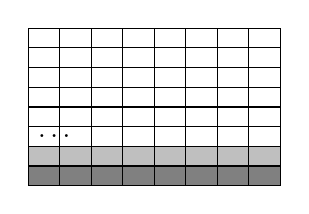
\begin{tikzpicture}
          \fill[gray] (0,0) rectangle (3.2, 0.25);
          \fill[lightgray] (0,0.25) rectangle (3.2, 0.5);
        \foreach \x in {0, 0.4, ..., 3.2} {
            \draw (\x, 0) -- (\x, 2);
        }
        \foreach \y in {0, 0.25, ..., 2} {
            \draw (0, \y) -- (3.2, \y);
        }
          \node[right] at (0, 0.625) {$\dots$};
    \end{tikzpicture}\]
    Аналогично доказательству~(\cref{integral-along-path}), в каждом горизонтальном прямоугольнике найдётся первообразная $F_j$, а дальше их надо сшить.
    Сшить несложно: вдоль горизонтального отрезка --- пересечения прямоугольничков --- $F_j\big|_{\dots} = F_{j+1}\big|_{\dots}$.
        Так как это --- первообразные вдоль пути, то они отличаются на константу. Значит, можно изменить все $F_j$ на константы так, чтобы их склейка была непрерывной функцией.

    Дальше надо проверить, что действительно получилась первообразная на квадрате.
        Выберем точку $(s, t) \in K$.
        Если точка попала внутрь какого-то прямоугольничка, то можно выбрать окрестность, лежащую внутри прямоугольничка, иначе чуть сложнее, но несильно.
    }
    }
    \theorem{
    Интегралы от замкнутой формы $\Phi$ по гомотопным замкнутым путям равны.
    \provehere{
    Определим $w(t) \coloneqq \int\limits_{\gamma_t}\Phi$ для всех $t \in [0, 1]$.

    Пусть $F$ --- первообразная для формы $\Phi$ вдоль гомотопии $\Gamma$. Понятно, что $w(t) = F(t, b) - F(t, a)$.

    Докажем, что $w$ локально постоянна на $[0, 1]$, следствием будет, что $w$ постоянна, что и требуется доказать.

    $\forall (\alpha, \beta) \in [0, 1] \times [a, b]$: $\exists \delta > 0$,  круг $U$ и первообразная $H_U$, такие, что
        \[\all{|\alpha - \alpha'| < \delta \\ |\beta - \beta'| < \delta} \then F(\alpha', \beta') = H_U(\Gamma(\alpha', \beta'))\]
    Пусть $U_1, U_2$ --- такие шары для $(t, b)$ и $(t, a)$ соответственно. \
    Тогда для $\tau$, достаточно близких к $t$, выполнено $w(t) = H_{U_1}(\Gamma(t, b)) - H_{U_2}(\Gamma(t, a))$.
    $H_1, H_2$ --- две первообразные в одной окрестности, они отличаются на константу, а $\Gamma(t, a) \equiv \Gamma(t, b)$, поэтому $w$ локально постоянна.
    }
    }
    \note{
    Если очень хочется, то можно соединить пути $\gamma_0: [a_0, b_0] \map \C$ и $\gamma_1: [a_1, b_1] \map \C$ гомотопией $\Gamma: K \map \C$, где $K \coloneqq \defset{(t, s)}{t \in [0, 1], s \in [a_t, b_t]}$ ($a_t, b_t$ --- какие-то непрерывные функции от $t$, такие, что $a_t < b_t$).
    }
    \section{Ряды Лорана}
    \emph{Ряд Лорана} $f(z)$ --- ряд вида $f(z) = \sum\limits_{n \in \Z}c_n (z - z_0)^n$.

    Говорят, что ряд Лорана сходится в точке $z$, если оба ряда $f_+(z) = \sum\limits_{n \ge 0}c_n (z - z_0)^n$ и $f_-(z) = \sum\limits_{n < 0}c_n (z - z_0)^n$ сходятся.

    Первый ряд степенной, имеется некий радиус сходимости $r_+$, такой, что $|z - z_0| < r_+ \then f_+$ сходится.
    При замене переменной $w \coloneq \frac{1}{z - z_0}$, $f_-(\nicefrac{1}{w})$ становится степенным рядом от $w$, сходящимся при $w < \frac{1}{r_-}$.

    Таким образом, ряд сходится абсолютно внутри <<кольца>> $\defset{z \in \C}{r_- < |z - z_0| < r_+}$:
    \[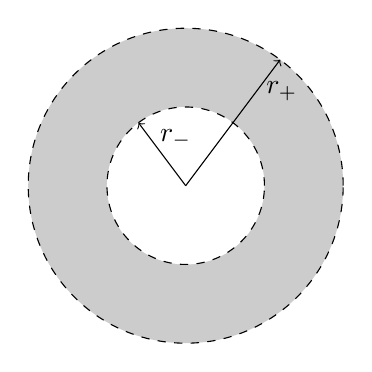
\begin{tikzpicture}
          \definecolor{lightgray}{rgb}{0.8,0.8,0.8}
          \fill[lightgray] (0, 0) circle (2);
          \fill[white] (0, 0) circle (1);
          \draw[->] (0, 0) -- (-0.6, 0.8) node[near end, right]{$r_-$};
          \draw[->] (0, 0) -- (1.2, 1.6) node[near end, right]{$r_+$};
          \draw[dashed] (0, 0) circle (2);
          \draw[dashed] (0, 0) circle (1);
    \end{tikzpicture}\]
    \theorem{
    Пусть $0 \le r_- < r_+ \le \infty$, функция $f$ голоморфна в <<кольце>> $K \coloneqq \defset{z \in \C}{r_- < |z| < r_+}$.

    Тогда $f$ представима в $K$ сходящимся рядом Лорана.
    \provehere{
    Пусть $z \in K$.
    Определим $\phi_z: K \map \C, \phi_z(\zeta) = \all{\frac{f(\zeta) - f(z)}{\zeta - z},&\zeta \ne z \\ f'(z),&\zeta = z}$.

    Согласно~(\cref{disposable-feature}), форма $\phi_z(\zeta)\d \zeta$ замкнута в $K$.

    Выберем $r, R \in \R$ так, что $r_- < r < |z| < R < r_+$.
    Для $\rho \in \R$ определим ${\gamma_\rho: [0, 2\pi] \map K, \gamma_\rho(t) \coloneqq \rho e^{it}}$.
    Пути $\gamma_R$ и $\gamma_r$ гомотопны, значит, $\int\limits_{\gamma_r}\phi_z(\zeta) \d \zeta = \int\limits_{\gamma_R}\phi_z(\zeta) \d \zeta$.
        А именно,
    \[\int\limits_{\gamma_R}\frac{f(\zeta) - f(z)}{\zeta - z}\d\zeta = \int\limits_{\gamma_r}\frac{f(\zeta) - f(z)}{\zeta - z}\d\zeta\]
    Преобразовывая, получаем
    \[\int\limits_{\gamma_R}\frac{f(\zeta)}{\zeta - z}\d\zeta - \int\limits_{\gamma_r}\frac{f(\zeta)}{\zeta - z}\d\zeta = f(z)\underbrace{\int\limits_{\gamma_R}\frac{1}{\zeta - z}\d\zeta}_{2\pi i} - f(z)\underbrace{\int\limits_{\gamma_r}\frac{1}{\zeta - z}\d\zeta}_{0}\]
    Тем самым, получили \emph{малую интегральную форму Коши для кольца}:
    \[f(z) = \frac{1}{2\pi i}\left(\,\int\limits_{\gamma_R}\frac{f(\zeta)}{\zeta - z}\d\zeta - \int\limits_{\gamma_r}\frac{f(\zeta)}{\zeta - z}\d\zeta\right)\]
    Осталось преобразовать дроби в ряды:
    \gather{
        \int\limits_{\gamma_R}\frac{f(\zeta)}{\zeta - z}\d\zeta = \int\limits_{\gamma_R}\frac{f(\zeta)}{(\zeta - z_0) - (z - z_0)}\d\zeta = \int\limits_{\gamma_R}\frac{1}{\zeta - z_0}\frac{f(\zeta)}{1 - \frac{z - z_0}{\zeta - z_0}}\d\zeta = \sum\limits_{j = 0}^{\infty}\int\limits_{\gamma_R}\frac{f(\zeta)}{(\zeta - z_0)^{j + 1}}\d\zeta \cdot (z - z_0)^j\\
        \int\limits_{\gamma_r}\frac{f(\zeta)}{\zeta - z}\d\zeta = \int\limits_{\gamma_r}\frac{f(\zeta)}{(\zeta - z_0) - (z - z_0)}\d\zeta = -\frac{1}{z - z_0}\int\limits_{\gamma_r}\frac{f(\zeta)}{1 - \frac{\zeta - z_0}{z - z_0}}\d\zeta = -\frac{1}{z - z_0}\sum\limits_{k = 0}^{\infty}\int\limits_{\gamma_r}f(\zeta)(\zeta - z_0)^k\d\zeta \cdot \frac{1}{(z - z_0)^{k}}
    }
    Сходимость степенная, имеется признак Вейерштрасса, можно поменять местами сумму и интеграл, поэтому все преобразования законны.

    При замене $j = -k - 1$, второе выражение преобразуется в форму
    \[-\sum\limits_{j = -1}^{-\infty}\int\limits_{\gamma_r}\frac{f(\zeta)}{(\zeta - z_0)^{j+1}}\d\zeta\cdot (z - z_0)^j\]
    Теперь можно заметить, что интегралы вдоль $\gamma_r$ и $\gamma_R$ равны, так как особенностей у интегралов --- слагаемых в ряде --- в кольце нет. Окончательно получаем
    \encircle{f(z) = \sum\limits_{j \in \Z}c_j (z - z_0)^j\text{, где }c_j = \int\limits_{|z - z_0| = \rho}\frac{f(\zeta)}{(\zeta - z_0)^{j + 1}}\d\zeta\text{ для любого $\rho \in (r_-, r_+)$}}
    }
    }
    \newlection{22 марта 2024 г.}
    Ряд Лорана $g(z) = \sum\limits-{j \in \Z}c_jz^j$ принято раскладывать на две части --- \emph{регулярную} $\sum\limits_{j \ge 0}c_j (z - z_0)^j$ и \emph{главную} $\sum\limits_{j < 0} c_j (z - z_0)^j$.

    Если ряд Лорана изучать в маленькой окрестности $z_0$, то главная часть асимптотически больше.
    Регулярная же сходится на всей комплексной плоскости.
    \section{Изолированные особенности голоморфных функций}
    Пусть область $G \subset \C, z_0 \in G$, $f$ задана и аналитична в $G \sm \{z_0\}$.
    Тогда говорят, что $f$ \emph{имеет особенность в $z_0$}.

    Возможны случаи:
    \numbers{
        \item $f$ ограничена вблизи $z_0$.

        Точка $z_0$ называется \emph{устранимой особенностью}, так как в силу~(\cref{singularities}) $\exists \lim\limits_{z \to z_0}f(z)$.
        \item $\lim\limits_{z \to z_0}|f(z)| = \infty$.

        Точка $z_0$ называется \emph{полюсом}.
        \item $f$ не имеет предела в $z_0$.

    Точка $z_0$ называется \emph{существенно особой точкой}.
    }
    \theorem{\label{singularities}
        В первом случае --- $f$ ограничена вблизи $z_0$ --- $f$ единственным образом продолжается до аналитической функции в области $G$.
        \provehere{
            Выберем $R > 0$ такой, что $B(z_0, R) \subset G$.
            $f$ разложится в некоторый ряд Лорана при $0 < |z - z_0| < R$.

            Запишем $c_j = \frac{1}{2\pi i}\int\limits_{0}^{2\pi}f(z + \rho e^{it})(\rho e^{it})^{-j-1} \cdot \rho e^{it}\d t$ и грубо оценим коэффициенты главной части ($j < 0$).
            Пусть $|f| \le C$ внутри круга $B(z_0, R)$ для некоторой константы $C$.
        \[|c_j| \le \frac{C}{2\pi}\int\limits_{0}^{2\pi}\rho^{-j}\d t = C \rho^{-j}\]
        Устремляя $\rho \to 0$, получаем $c_j = 0$.
            Тем самым, $f$ раскладывается в ряд Тейлора в окрестности $z_0$.
        }
    }
    Запишем несколько другую классификацию особенностей точки, опирающуюся на ряд Лорана $f(z) = \sum\limits_{j \in \Z}c_j (z - z_0)^j$.
    \begin{enumerate}[I]
    \item При всяком $j < 0$: $c_j = 0$.
    \item Множество $\mathcal{A} \coloneqq \defset{j < 0}{c_j \ne 0}$ конечно.
    \item Множество $\mathcal{A} \coloneqq \defset{j < 0}{c_j \ne 0}$ бесконечно.
    \end{enumerate}
    Понятно, что I эквивалентно 1.
    \theorem{
    На самом деле, II $\iff$ 2, III $\iff$ 3.
    \provebullets{
        \item[II $\then$ 2] Пусть $k = -\min \mathcal{A}$.
    \[f(z) = \frac{c_{-k}}{(z - z_0)^k} + \frac{c_{-k+1}}{(z - z_0)^{k-1}}\cdots + c_0 + \sum\limits_{j > 0}c_j (z - z_0)^j\ = \frac{1}{z - z_0}^k\left(c_{-k} + c_{-k + 1} + \cdots \right) = \frac{g(z)}{(z - z_0)^k}\]
    При этом $g(z_0) \ne 0$ и $g(z)$ аналитична. Тем самым, $\lim\limits_{z \to z_0}|f(z)| = \infty$.
    \item [2 $\then$ II] Положим $h(z) \coloneqq \frac{1}{f(z)}$ в некоторой окрестности $z_0$.

    $h$ аналитична при $z \ne z_0$, и $\lim\limits_{z \to z_0}h(z) = 0$, значит, $h$ имеет устранимую особенность в $z_0$.
    \comment{Может что-то пропустил.}
        Пусть $k$ --- наименьший номер, такой, что $b_k \ne 0$, где $b_k$ --- коэффициент из разложения $h$ в ряд Тейлора:
        \[h(z) = b_k (z - z_0)^k + b_{k+1}(z - z_0)^{k + 1}\cdots + \cdots = (z - z_0)^k(b_k + b_{k+1}(z - z_0) + \cdots) = (z - z_0)^k \cdot u(z)\]
    $u$ аналитична вблизи $z_0$, и $u(z_0) = b_k \ne 0$.
    \[f(z) = \frac{1}{(z - z_0)^k}\frac{1}{u(z)} = \frac{1}{(z - z_0)^k}\left(c_0 + c_1(z - z_0) + \cdots\right)\]
    Почленно деля, действительно получаем, что $f(z)$ имеет конечное число ненулевых членов в разложении в ряд Лорана.
    }
    }
    Пусть $z_0$ --- полюс $f$, $k \coloneqq -\min\defset{j < 0}{c_j \ne 0}$.
    Число $k$ называется \emph{порядком} полюса $z_0$.

    Если же $g$ аналитична в $z_0, g(z_0) = 0, g \not\equiv 0$, то $g(z) = \sum\limits_{j \ge 0}a_j (z - z_0)^j$, положим $l \coloneqq \min\defset{j}{a_j \ne 0}$.
    Число $l$ --- \emph{порядок} $f$.
    \fact{$f$ имеет полюс порядка $k$ в $z_0 \iff \frac{1}{f}$ имеет ноль порядка $k$ в $z_0$.}
    \intfact[Теорема Пикара]{
    Пусть $z_0$ --- существенно особая точка аналитической функции $f$. Тогда $\forall \eps > 0: f(\defset{z}{0 < |z - z_0| < \eps})$ есть $\C$, кроме, может быть, двух точек.
    }
    Мы докажем более простой вариант теоремы Пикара.
    \theorem[Сохоцкий]{
        Пусть $z_0$ --- существенно особая точка аналитической функции $f$. Тогда $\forall \eps > 0: \mathcal{B} \coloneqq f(\defset{z}{0 < |z - z_0| < \eps})$ плотно в $\C$.
    \provehere{
    От противного: пусть $\exists w_0 \notin \overline{B}$, то есть $\exists \delta > 0: B(w_0, \delta) \cap \mathcal{B} = \o$.

    Определим \begin{align*}h: B(z_0, \eps) \sm \{z_0\} &\map \C\\ z &\mapsto \frac{1}{f(z) - w_0}\end{align*}
        Хотя $h$ и имеет особенность при $z = z_0$, но $h$ ограничена, то есть особенность устранима.
        $f(z) = \frac{1}{h(z)} + w_0$, и так как $h$ аналитична в $z_0$, то особенность в $z_0$ --- то ли тоже устранимая особенность, то ли полюс, но уж никак $z_0$ --- не существенно особая точка.
    }
    }
    \example{
    Возьмём $\int\limits_{0}^{\infty}\frac{\sin x}{x}\d x$.
    У подынтегральной функции в нуле особенность устранимая, а с бесконечностью есть некоторые проблемы.
        Впрочем, избавимся и от нуля в области интегрирования:
        \[\int\limits_{0}^{\infty}\frac{\sin x}{x}\d x= \lim\limits_{\eps \to 0, R \to \infty}\int\limits_{\eps}^{R}\frac{\sin x}{x}\d x \circlesign{=} \]
        Запишем формулу Эйлера $e^{ix} = \cos x + i\sin x$. Интегрируя по всей оси $\frac{\cos x}{x}$, мы поучим нуль из-за нечётности, поэтому можно продолжить равенство так:
    \[\circlesign{=}\frac{1}{2i}\lim\limits_{\eps \to 0, R \to \infty}\int\limits_{\eps < |x| < R}\frac{e^{ix}}{x}\d x\]
    Теперь перейдём к функции, аналитической в комплексной плоскости: $\phi(z) \coloneqq \frac{e^{iz}}{z}$.

    Введём путь $\Gamma = [\eps \to R] \cdot \gamma_R \cdot [-R \to -\eps] \to \gamma_\eps$, где $[a \to b]$ --- путь, проходящий отрезок $[a, b]$ в направлении от $a$ к $b$, а $\all{\gamma_R(t) = R e^{it},&t \in [0, \pi] \\ \gamma_\eps(t) = \eps e^{i(\pi - t)},&t \in [0, \pi]}$.
    \[\int\limits_{\gamma_\eps}\phi(z)\d z = \int\limits_{0}^{\pi}\frac{e^{i \eps e^{i(\pi-t)}}}{\eps e^{i (\pi - t)}}\eps i e^{i(\pi - t)}\d t = \int\limits_{0}^{\pi}i e^{i \eps e^{i(\pi-t)}}\d t \overset{\text{подынтегральное выражение равномерно сходится к $i$.}}{\underset{\eps \to 0}\Map} -i\pi\]
    \[\int\limits_{\gamma_R}\phi(z)\d z = \int\limits_{0}^{\pi}\frac{e^i R e^{it}}{R e^{it}}R i e^{it}\d t = i \int\limits_{0}^{\pi}e^{i R e^{it}}\d t\]
    Оценим $e^{i R e^{it}} = e^{i R \cos t - R \sin t} = e^{i R \cos t} \cdot e^{-R \sin t}$.
        По теореме Лебега о мажорируемой сходимости интеграл по $\gamma_R$ будет \textbf{нулём}.
    \comment{...}
    }
    Этот интеграл получилось так взять, так как у $\phi$ была особенность в нуле, и мы её обошли.
    А иногда особенности находятся внутри пути интегрирования, в таком случае пригождается \emph{формула в вычетах}.
    \section{Вычеты}
    Пусть $f$ задана и голоморфна в $G \sm \{z_0\}$, где $G$ --- область, $z_0 \in G$ --- изолированная особенность.

    Вблизи $z_0$ $f$ раскладывается в ряд Лорана $f(z) = \sum\limits_{j \in \Z}c_j (z - z_0)^j$.
    \definition[Вычет функции $f$ в точке $z_0$]{
        Коэффициент $c_{-1}$, обозначается $\Res_{z_0}f$.
    }
    Этот коэффициент так важен, так как у $c_j (z - z_0)^j$ при $j \ne -1$ имеется первообразная в $G$, и при интегрировании по окружности, обходящей $z_0$, пропадут все коэффициенты ряда Лорана, кроме вычета.
    \subsection{Как вычислять вычеты}
    У нас есть формула для вычисления коэффициентов ряда Лорана, но она получается интегрированием, а мы как раз и хотим использовать вычеты, чтобы уметь удобно интегрировать.
    Поэтому иногда пригождаются следующие частные случаи:
    \bullets{
    \item Пусть $z_0$ --- полюс функции $f$ степени $k$:
    \[f(z) = \frac{c_{-k}}{(z - z_0)^k} + \frac{c_{-k + 1}}{(z - z_0)^{k - 1}} + \cdots + \frac{c_{-1}}{(z - z_0)} + f_+(z)\]
    где $f_+$ --- аналитическая вблизи $z_0$.

    Домножая $f$ на $(z - z_0)^k$, получаем аналитическую \[(z - z_0)^k f = c_{-k} + c_{-k + 1}(z - z_0) + \cdots + c_{-1}(z - z_0)^{k - 1} + (z - z_0)^k \cdot f_+(z)\]
    Теперь можно найти $\Res_{z_0}f$ по формуле: $\Res_{z_0}f = \frac{1}{(k - 1)!}\cdot \left(\frac{\d}{\d z}\right)^{k-1}\left[(z - z_0)^k f(z)\right]\Big|_{z = z_0}$.
    \item Пусть $k = 1$ --- у $f$ имеется полюс первого порядка. Тогда дифференцировать не надо, и формула вырождается в
    \[\Res_{z_0}f = \lim\limits_{z \to z_0}(z - z_0)f(z)\]
    \item Возьмём ещё более частный случай: $f(z) = \frac{g(z)}{h(z)}$, где $g, h$ аналитичны в окрестности $z_0$, $g(z_0) \ne 0$, а $h$ имеет простой нуль в $z_0$ (нуль кратности $1$).
    \[\Res_{z_0}f = \lim\limits_{z\to z_0}\frac{f(z)(z - z_0)}{h(z)} = \lim\limits_{z\to z_0}g(z)\frac{z - z_0}{h(z) - h(z_0)} = \frac{g(z)}{h'(z)}\]
    }
    \subsection{Индекс замкнутого пути относительно точки}
    Пусть $G \subset \C$ --- область, $\Phi$ --- замкнутая дифференциальная форма в $G$.
    Пусть $\gamma_1, \dots, \gamma_n$ --- какие-то замкнутые пути с носителем в $G$.
    Обозначим $\Gamma = \{\gamma_1, \dots, \gamma_n\}$.

    Определим интеграл от формы $\Phi$ по данной совокупности путей $\int\limits_{\Gamma}\Phi \bydef \sum\limits_{j = 1}^{n}\int\limits_{\gamma_j}\Phi$.

    Назовём систему путей $\Gamma$ \emph{правильной}, если для всякой аналитической функции $f$ в $G$: $\int\limits_{\Gamma}f(z)\d z = 0$.
    \examples[Правильные системы путей]{
    \item $|\Gamma| = 1$. Если $\gamma_1$ гомотопен тождественному, то $\Gamma$, конечно, правильная.
    \item В частности, любой замкнутый путь в односвязной области формирует правильную систему из одного пути.
    \item Пусть в кольце имеются два пути $\gamma_1, \gamma_2$, обходящие концентрические окружности в противоположных направлениях.
    Тогда $\{\gamma_1, \gamma_2\}$ --- правильная система, так как $\gamma_1 \sim \gamma_2^-$.
    \item Рассмотрим область с двумя дырками, и тремя путями --- ну тут без картинки точно не обойтись.
    % типа один путь обходит обе дырки, два других --- по однйо дырке в противоположном направлении, и мы проводим три отрезка, и раскладываем пути в сумму двух стягиваемых
    }
    Пусть $\gamma$ --- петля в $\C$, $z_0 \notin \Image(\gamma)$.
    \definition[Индекс пути $\gamma$ относительно $z_0$]{
    Значение интеграла $\frac{1}{2\pi i}\int\limits_{\gamma}\frac{\d z}{z - z_0}$.
    Обозначается $\Ind_{z_0}\gamma$.
    }
    Это определение очевидным образом распространяется на систему путей: $\forall \gamma_j \in \Gamma: z_0 \notin \Image(\gamma) \then$ определён $\Ind_{z_0}\Gamma \bydef \sum\limits_{j = 1}^{n}\frac{1}{2\pi i}\int\limits_{\gamma_j}\frac{\d z}{z - z_0}$
    \properties[Свойства индекса, докажем потом]{
    \item $\Ind_{z_0}\gamma \in \Z$.
    \item Функция $[z_0 \mapsto \Ind_{z_0}\gamma]$ постоянна на каждой компоненте связности $\C \sm \Image(\gamma)$.
    \item На неограниченной компоненте связности $\C \sm \Image(\gamma)$ индекс равен нулю.
    }
    \theorem[Формула вычетов]{
        Пусть $G \subset \C$ --- область, $\Gamma$ --- правильная система путей в $G$, $f: G \sm \{z_1, \dots, z_k\} \map \C$ --- аналитическая функция, и $z_1, \dots, z_k$ --- её полюса.
        Если все точки $z_j$ не лежат на носителе системы путей $\Gamma$, то
        \encircle{\int\limits_{\Gamma}f(z)\d z = 2\pi i\left(\sum\limits_{j = 1}^{k}\Res_{z_j}f \cdot \Ind_{z_j}\Gamma\right)}
    \provehere{
    Пусть $g_1, \dots, g_k$ --- главные части рядов Лорана для $f$ в точках $z_1, \dots, z_k$ соответственно.
    Тогда функция $h(z) \coloneqq f(z) - g_1(z) - \dots - g_k(z)$ --- аналитическая функция в области $G$.

    Так как $\Gamma$ --- правильная, то $\int\limits_{\Gamma}h(z)\d z = 0$. Тем самым, мы получили
    \[\int\limits_{\Gamma}f(z)\d z = \sum\limits_{j = 1}^{k}\int\limits_{\Gamma}g_j(z)\d z\]
    Посчитаем $\int\limits_{\Gamma}g_j(z)\d z$. Распишем \[g_j(z) = \frac{\Res_{z_j}g}{z - z_j} + \frac{a_1}{(z - z_j)^2} + \dots + \frac{a_{s-1}}{(z - z_j)^s}\]
    У всех слагаемых, кроме первого, есть первообразная, значит, $\int\limits_{\Gamma}g(z)\d z = (\Res_{z_j}f)2\pi i \cdot \Ind_{z_0}\Gamma$ (очевидно, $\Res_{z_j}g_j = \Res_{z_j}f$).
    }
    }
    \comment{На самом деле, теорема верна и для существенно особых точек, только надо чуть больше слов сказать, может, я их напишу попозже.}
\end{document}
